\documentclass[withoutpreface,bwprint]{cumcmthesis} %去掉封面与编号页,电子版提交的时候使用。
\usepackage{bm}
\usepackage{appendix}
\usepackage[framemethod=TikZ]{mdframed}
\usepackage{url}   % 网页链接
\usepackage{subcaption} % 子标题
\usepackage{array}
\usepackage{graphicx}
\usepackage{caption}
\usepackage{float}
\usepackage{natbib}
\usepackage{enumitem}
\usepackage{booktabs}
\usepackage{pdfpages}
\usepackage{graphicx}

\usetikzlibrary{decorations.pathreplacing} % 用于添加大括号的库

\begin{document}
\title{编者注}

\maketitle
首先恭喜大家通过了前面的考核,选择了加入视觉/算法组。   

机器视觉是当前计算机发展的一个重要的研究方向,它旨在实现机器人对环境进行更加详细地感知。
由于可见光在成像方面清晰度、成像速度方面等具有很好的优势,因此机器视觉的研究也逐渐成为计算机视觉领域的研究热点。
在技术发展过程中,计算机视觉的技术可以大体分为两个技术方向,即图像处理与机器学习。

\textbf{图像处理}是指通过计算机对图像进行分析、处理、识别、理解等,从而实现对图像的高效、准确的描述、分析和理解。
主要的方法是通过计算机算法对图像进行处理,如图像增强、图像分割、图像检索、图像配准、图像修复、图像检索、图像分类、图像检索、图像压缩等。
在实际的应用场景中具有性能开销小,运算速度快,开发成本低等优点。

\textbf{机器学习}是指通过神经网络对图像进行分析。今年来随着深度学习和卷积神经网络的发展,机器学习技术也越来越多的应用于计算机视觉中。
机器学习的主要方法是通过训练数据对计算机模型进行训练,使计算机能够对未知数据进行预测、分类、聚类、回归等。
在图像处理中,机器学习可以应用于图像分类、目标检测、图像分割、图像检索、图像配准、图像修复等。
也涌现出了一大批优秀的物体识别算法,如YOLO等。

在实际的应用场景中,两种方法不是互相孤立的,而是需要我们相互结合,取长补短,才能达到更好的效果。除此之外,
光有计算机视觉也是远远不够的,
在现实的生产生活中,制造机器人主要的目的是为了达到自动化,面对真正的项目,
一般都是在一个miniPC中实现控制理论和多个数据融合处理,之后配合若干下位机进行自动化地完成任务。
所以代码、算法以及一些控制理论只是我们的工具,真正的目标是多感官的融合和自动化的控制。

俗话说“工欲善其事,必先利其器”,只有我们对基本的编程语言,对计算机的行为逻辑,对硬件作用与联系有着深刻的理解,
才能更好地理解每一种算法的特点,更好地洞悉每种操作背后的原理。从而应用到实际,切实地提高我们的创新能力和解决问题的能力。

在我们的培训中,我们将由浅入深,细致地为大家讲解机器视觉的知识,让大家能够更加深入地理解图像处理与机器学习的原理,
并运用到实际的项目中,提升自己的能力。在接下来的学习中,我们将更加注重理论知识的学习,重点讲解机器视觉的理论基础,
以及如何运用到实际的项目中。

送同学们一首我非常喜欢的诗:

\textbf{天高云淡, 望断南飞雁。 不到长城非好汉, 屈指行程二万。} 

\textbf{六盘山上高峰, 红旗漫卷西风。 今日长缨在手, 何时缚住苍龙?}

最后,祝大家学习愉快,工作顺利!

\newpage

\tableofcontents
\footnote{表星号的内容属于选修内容}
\newpage

\section{走进Linux系统}

\section{现代C++技术}
\subsection{走进面向对象编程:类}

\subsubsection{类的基本概念}

类是\textbf{面向对象}(OB,Object-Oriented)最基本的概念,也是C++区别于C语言的重要特征。
面向对象编程的基本思想是抽象出对象,将对象作为程序的基本单元,通过消息传递来进行通信和协作。
对象是类的实例,具有状态和行为,状态存储在对象的数据成员中,行为由对象的方法实现。
对象通过消息传递进行通信,对象之间可以互相发送消息,并处理消息。
面向对象编程的优点是代码的可重用性、可扩展性和可维护性都得到了提高。

在C++中,类是一种抽象数据类型,它定义了对象的行为和状态,并提供了对这些数据的访问接口。
类可以包含数据成员、成员函数、构造函数、析构函数等,这些成员构成了类的接口。
类可以派生出新的类,从而实现代码的重用和扩展。

\begin{tcode}
class ClassName{        //类名
    public:             //修饰限定符public
        ClassName();    //构造函数
        ~ClassName();   //析构函数
        void memberFunction();  //成员函数
    private:                    //修饰限定符private
        int dataMember;         //数据成员
        void privateFunction(); //私有成员函数
}    

\end{tcode}

\begin{enumerate}
    \item \textbf{构造函数和析构函数}:类的构造和析构过程,它们负责对象的初始化和释放,其特点是其函数名与类名相同,没有返回值。
    \item \textbf{成员函数}:实现类的行为,它们实现了类的功能。
    \item \textbf{数据成员}:存储类的数据信息。
\end{enumerate}
\begin{center}

    \begin{tabular}{cc}
        \hline
        修饰限定符 & 作用 \\
        \hline
        private & 只能被类的成员函数使用或调用 \\
        public & 可以被类外的其他函数或派生类中函数调用 \\
        protected & 只能被类的成员函数和派生类使用或调用 \\ 
        \hline
        
    \end{tabular}
\end{center}

% 类可以派生出新的类,派生类可以继承基类的所有成员,并可以添加新的成员。
% 派生类可以重写基类中的成员函数,从而实现新的功能。
% 派生类可以重载基类中的运算符,从而实现新的运算。

面向对象编程的实现方式有多种,包括面向过程、基于消息的、基于事件的、面向对象设计模式等。
面向过程的实现方式是将数据和函数分离,通过函数调用来实现对象之间的通信。
基于消息的实现方式是通过消息传递来实现对象之间的通信,消息可以是函数调用、事件、数据等。
基于事件的实现方式是通过事件驱动模型来实现对象之间的通信,事件可以是用户操作、时间事件、状态变化等。

\subsubsection{静态和友元}

静态成员是指在类外部定义的变量和函数,它属于整个类,而不是类的对象。
静态成员可以\textbf{被类的所有对象}共享,因此可以实现一些全局变量的功能。
静态成员的声明和定义都在类的外部,因此在类的声明中不需要加$static$关键字。

需要特别注意的是,静态变量的定义必须在实例化之前。静态成员的生命周期和整个程序的生命周期是相同的,因此静态成员的构造函数和析构函数只会被调用一次。
\begin{enumerate}
    \item 友元函数:友元函数可以访问类的私有成员,但不能调用类的私有成员函数。
    \item 静态成员:静态成员可以被类的所有对象共享,因此可以实现一些全局变量的功能。
    \item 静态变量:静态变量的定义必须在实例化之前。静态成员的生命周期和整个程序的生命周期是相同的,因此静态成员的构造函数和析构函数只会被调用一次。
\end{enumerate}

\begin{tcode}
class ClassName {
    public:
        ClassName() = default;
    
        ~ClassName() = default;
    
        static void memberFunction();   //成员函数
        static int dataMember;          //数据成员
        friend void FriendFunction(int a, int b);//友元函数定义
    private:                            //修饰限定符private
        static void privateFunction();  //私有成员函数
};
        
void FriendFunction(int a, int b){ //友元函数实现时,不可以添加类的作用域
    std::cout << "你调用了友元函数";
}
        
int ClassName::dataMember = 10; //静态变量只能在类的实例化之前定义
        
int main(int argc, char *argv[]) {
    ClassName obj1, obj2;
    cout << obj1.dataMember << endl;
    cout << obj2.dataMember;
        
    return 0;
}

\end{tcode}

有时,我们希望某个函数可以访问类的私有成员,但又不希望它成为类的成员函数。
这时,我们可以将函数声明为友元函数,并在类的声明中加上$friend$关键字。
友元函数可以访问类的私有成员,但不能调用类的私有成员函数。

\textbf{需要注意的是,不属于类,它破坏了类的封装性,因此不建议使用!}

\subsubsection{函数重载}
\textbf{函数重载(overload)}是指在同一个作用域中,存在多个同名函数,但它们的参数个数或参数类型不同。
函数重载的作用是为了使程序更加灵活,提高代码的可读性和可维护性。

在C++中,函数重载的规则是:
\begin{enumerate}
    \item 函数名相同;
    \item 参数个数不同;
    \item 参数类型不同。
\end{enumerate}

\begin{tcode}
class ClassName {
public:
    ClassName() = default;

    ~ClassName() = default;

    int CalSum(int a,int b){
        return a+b;
    }

    double CalSum(double a,double b){
        return a+b;
    }
};

int main(int argc, char *argv[]) {
    ClassName obj;
    cout << obj.CalSum(1,2) << endl;
    cout <<  obj.CalSum(1.5,2.5);

    return 0;
}
\end{tcode}

在上例中,CalSum函数的两个版本都可以接受两个参数,但它们的返回值和参数类型不同。
因此,我们可以实现两个函数的重载,使得程序更加灵活。在执行函数时,编译器会根据函数的调用情况,自动选择最匹配的函数版本。

\textbf{构造函数的类型:}

\begin{enumerate}
    \item 默认构造:默认构造函数是指没有参数的构造函数,它会创建一个对象,并对其进行初始化。
    \item 含参构造:含参构造函数是指有参数的构造函数,可以根据参数的值对对象进行初始化。
    \item 拷贝构造:拷贝构造函数是指将一个对象拷贝到另一个对象时,会调用拷贝构造函数。
\end{enumerate}

\begin{tcode}
#include<iostream>
#include<string>
class ClassName {
public:
    ClassName():member(1) //初始化列表
    {std::cout << "你调用了默认构造函数" << std::endl;}
    ClassName(std::string& str) 
    {std::cout << "你调用了含参构造函数,参数是" << str << std::endl;member=2;}
    ClassName(ClassName &obj) //这里必须是引用传参,思考一下为什么
    {std::cout << "你调用了拷贝构造函数" << std::endl;
    this->member = obj.member;}
    ~ClassName() = default;

    int member;
};

int main(int argc, char *argv[]) {
    ClassName obj1;
    std::string str = "Hello World";
    ClassName obj2(str);
    obj1.member = 10;
    ClassName obj3(obj1);

    std::cout << "obj1:" << obj1.member << std::endl;
    std::cout << "obj2:" << obj2.member << std::endl;
    std::cout << "obj3:" << obj3.member << std::endl;

    return 0;
}
\end{tcode}
有一些tips可以快速设置构造函数
\begin{tcode}
ClassName() = default;              //默认构造函数,使用默认的方式
ClassName(ClassName& obj) = delete; //禁止拷贝构造,单例实现对象
\end{tcode}
\textbf{运算符重载:}

在C++中,类提供了一个接口,可以将运算符进行重载,从而实现对类更加灵活的操作。
运算符重载的语法如下:

\begin{tcode}
[返回值] operator [操作符] ([参数列表]) {
    //操作符的实现
}
\end{tcode}

示例:

\begin{tcode}
class ClassName {
    public:
        ClassName():a(1),b(2) {}
    
        ClassName& operator+(ClassName& obj){//重载加法运算符
            this->b += obj.b;   //this指针,指向自己
            this->a += obj.a;
            std::cout << "这里执行过了" << std::endl;
            return *this;   //*this表示当前对象的引用
        }
     
        //重载流插入运算符,思考一下为什么是这样写?
        friend std::ostream& operator<<(std::ostream& out, ClassName& obj);
    
        int a;
        int b;
    };
    
    std::ostream& operator<<(std::ostream& out, ClassName& obj){
        out << "a:" << obj.a << " b:" << obj.b << std::endl;
        return out;
    }
    
    int main(int argc, char *argv[]) {
        ClassName obj1;
        ClassName res = obj1 + obj1;
        std::cout << res;
    
        return 0;
    }
\end{tcode}

\textbf{$this$指针}是一个隐指针,指向这个类本身。
在类的成员函数中,$this$指针可以用来访问类的成员变量和成员函数。
在类的构造函数中,$this$指针可以用来初始化类的成员变量。
一般情况下,$this$指针可以不写,编译器会自动生成。但是有些情况,处于项目代码可读性的目的,会写显性的$this$指针。
此外,类中成员函数的第一个参数必须是$this$指针,表示当前对象的引用。这也是类的成员函数的调用方式。在后面我们会详细解释类的执行方式,此处略去不表。

\subsubsection{类的继承}
类的继承是面向对象编程的重要特征之一,它允许创建新的类,从而继承基类的成员,并添加新的成员。

\begin{figure}[H]
    \centering
    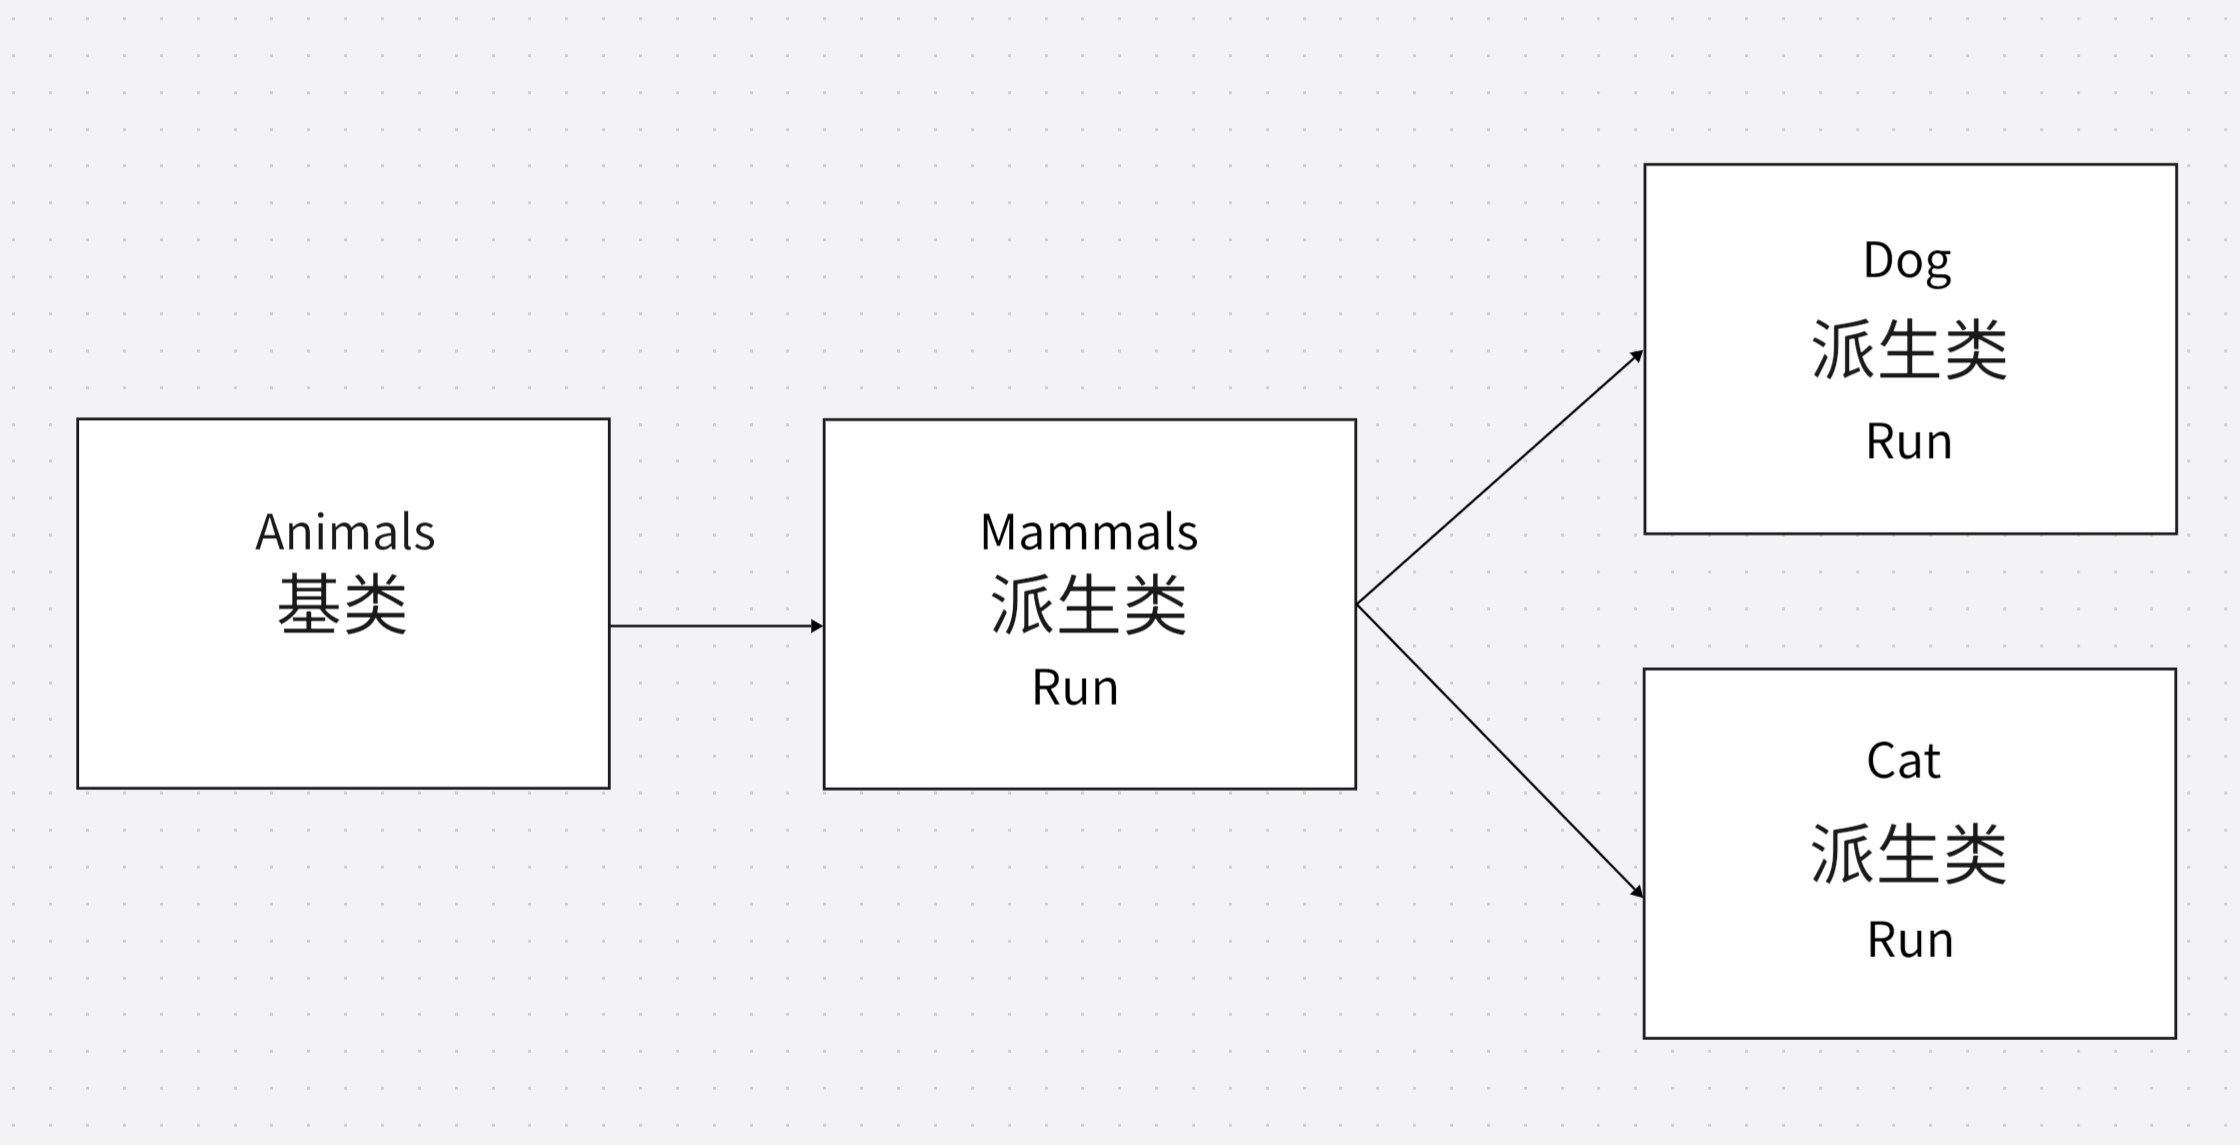
\includegraphics[width=0.7\textwidth]{A111.png}
    \caption{类的继承} % 图片标题
    \label{fig:A111} % 图片标签,用于引用
\end{figure}

如图\ref{fig:A111}所示,派生类从基类中继承了数据成员和成员函数,并可以添加新的成员。
派生类可以重写基类中的成员虚函数,从而实现新的功能。
派生类可以重载基类中的运算符,从而实现新的运算。

\begin{center}
\textbf{继承的三种方式:}

    \begin{tabular}{cccc}
        \hline
        访问 & public & private & protected \\
        \hline
        同一个类 & yes & yes & yes \\
        派生类 & yes & no & yes \\
        类外部 & yes & no & no \\ 
        \hline
        
    \end{tabular}
\end{center}

继承可以用下面的写法实现:

\begin{tcode}
class Shape {//这个基类只含有纯虚函数,又叫做抽象类
public:
    Shape() = delete;
    Shape(double A):Area(A)
    {std::cout << "基类的构造函数已经被调用" << std::endl;}
    virtual double calArea() = 0; //这里是纯虚函数,也可以使用普通函数
    double Area;
};

class Rectangle
        : protected Shape{
public:
    Rectangle() = delete;
    Rectangle(double a,double b):a(a),b(b),Shape(a*b)
    {std::cout << "Rectangle类的构造函数已经被调用,面积为" << Area << std::endl;}
    double a;
    double b;
    double calArea() override{  //重写基类的函数
        return a*b;
    }

};

class Circle
        :Shape{
public:
    Circle() = delete;
    explicit Circle(double r):r(r),Shape(3.14*r*r)
    {std::cout << "Circle类的构造函数已经被调用,面积:" << Area << std::endl;}
    double r;
    double calArea() override{
        return 3.14*r*r;
    }

};

int main(int argc, char *argv[]) {
    Circle circle(1.0);
    Rectangle rect(1.0,2.0);
    return 0;
}
\end{tcode}


 \subsubsection{模版}
在开发过程中,我们可能会遇到这样的场景,我们有一个函数或者类,但是它只适用于特定的数据类型,
比如$int$或者$double$。为了实现对这两种类型都可以调用函数,
就会遇到需要复制一遍代码,但是这样做就造成了代码冗余,不利于维护。这时候就需要用到模版($template$)。

模版是C++中一个重要的特性,它允许我们定义一个类或函数,使其可以接受不同的数据类型或者不同的参数。
模版的定义和使用都比较复杂,这里只介绍最基本的用法。
使用$class$关键字声明类型,使用具体的类型声明参数
\textbf{函数模版}的语法如下:
\begin{tcode}
template<class T>
T function(T a){
    return a;
}

auto funcPtr = function<int>;
template<int A>
int function(){
 return A;
}

auto funcPtr = function<2>;
template<class T,T A>
T function(){
 return A;
}
auto funcPtr = function<int,2>;
\end{tcode}

 这里的$class \quad T$表示一种数据类型,可以是任意类型。
 在函数的定义中,$T$可以作为函数的参数,也可以作为函数的局部变量。在使用函数模板时,需要首先进行函数的实例化。

\begin{tcode}
//调用的时候实际上分为两步,实例化和调用
function<int>(10);
function<double>(20.0);
//在编译器可以推导出类型的时候可以不加<>
auto a = function(1.0);
//在无法推导的时候,要先进行实例化
std::function<int(int)> ptr = function<int>;
\end{tcode}

模版的优点:
\begin{enumerate}
    \item 代码重用性高:可以定义一个通用的函数,然后根据需要实例化不同的类型,实现代码的重用。
    \item 类型安全:模版可以保证类型安全,避免类型错误。
    \item 效率高:模版可以提高效率,因为编译器可以对代码进行优化。
\end{enumerate}

\textbf{类模版}:
类模板的语法和函数模板类似,只不过在类名而不是函数名前面加上关键字$template$。
在普通类中也可以添加成员函数模版,只需要在函数名前面加上关键字$template$即可。

\begin{tcode}
template<class T1,class T2>
class A{
    A() = default;
    ~A() =default;
    T1 val;
    T2 id;
    T1 function(T1* a, T2& b){
        return *a+b++;
    }
};
\end{tcode}

在$template$后面,可以定义多个类型参数,用逗号分隔。需要注意的是,在类中的函数模版需要再头文件中实现,
也就是说,模版的声明和实现不可以分离,否则会出现很多问题。
对于类模板也可以实现继承和多态,与普通类相同,这里不在展开,感兴趣的同学可以自行探索。

\textbf{模板的实例化}:
模板的实例化指的是将模板定义和具体的类型绑定在一起,生成一个具体的类或函数。
在类的实例化时,$<>$的内部需要填写一个可以推导出的数据类型,编译器会根据类型推导出模板的具体类型。
一般来说,实例化有以下几种方式:

\begin{enumerate}
    \item 具体类型:如$int$,$double$等基本类型,$struct$,$class$,$union$等复合数据类型,$int*$,$double\&$等指针和引用类型
    \item 编译期可以确定的常数:字面常量,宏,$constexpr$
    \item 显示实例化:在编译时,通过命令行指定具体的类型
\end{enumerate}

除此之外,还有一种变参模版,它可以接受任意数量的类型参数,但是在实例化时,必须指定具体的类型。
这种情况比较复杂,这里不在展开。感兴趣的同学自行探讨:

\url{https://blog.csdn.net/fl2011sx/article/details/128077440}


\subsection{魔法代码:C++17}


随着时代的发展和项目变得越来越复杂,人们创造了一系列新的代码特性,其中一些特性在C++11和C++17中被引入,
在不熟悉这些特性的人看来,这些代码看上去显得十分无厘头,甚至有些难以理解。本章将介绍C++11和C++17中引入的一些新的代码特性,
并通过实例来说明它们的用法。
\subsubsection{lambda表达式}

\textbf{指名初始化(Designated Initializers)}是一种初始化聚合类型(Aggregate Types)成员的方式,
这种方式允许你指定每个成员的初始化值,而不必按照成员在聚合类型中的声明顺序进行初始化。
这种方式在C++11标准中被引入。他的语法很简单:

\begin{tcode}
//类型名 对象名{成员名1 = 初始值1, 成员名2 = 初始值2,...};
struct Foo {int a, b};
Foo foo = {.b = 3, .a = 1};
\end{tcode}

\textbf{匿名函数(anonymous function)}是一种在程序中定义的函数,它没有名字,只能在运行时创建。C++11引入了lambda表达式,
它是一种更简洁的语法,可以用来创建匿名函数。lambda表达式的语法如下:

\begin{tcode}
完成版:[捕获列表](参数列表) mutable throw(异常列表) -> 返回值 {函数体}
简化版:[捕获列表](参数列表) {函数体}
\end{tcode}    

\begin{enumerate}
    \item 捕获列表:捕获列表可以用来捕获外部作用域中的变量,使得lambda表达式可以访问这些变量。捕获列表的语法如下:
    \item 参数列表:参数列表定义了lambda表达式的参数,可以有0到多个参数。
    \item mutable[可选]:mutable关键字用来声明lambda表达式的捕获列表中的变量是可修改的。
    \item throw(异常列表)[可选]:throw关键字用来指定lambda表达式可能抛出的异常。
    \item 返回值:返回值定义了lambda表达式的返回类型。
    \item 函数体:函数体定义了lambda表达式的主体,可以是一条表达式或多条语句。
\end{enumerate}

\begin{tcode}
#include<iostream>
#include<functional>

template<class T>
void sort(T* array,int n,std::function<bool(T&,T&)> compare){
    for(int i=0;i<n;i++){
        for(int j=i;j<n;j++){
            if(!compare(array[i],array[j])){    //为false时,交换(按照指标降序)
                std::swap(array[i],array[j]);
            }
        }
    }
}

typedef struct Block{
    char ch;
    int id;
}Block;

int main(int argc, char *argv[]) {
    auto sum = [](int a,int b){
        return a+b;
    };

    std::cout << sum(1,2) << std::endl;

    Block blocks[5]={{'a',2},{'d',4},{'q',1},{'t',7},{'s',-1}};
    sort<Block>(blocks,5,[](Block& a1,Block a2){//lambda表达式作为参数传递
        return a1.id > a2.id;
    });
    for(int i=0;i<5;i++){
        std::cout << "ch:" << blocks[i].ch << "  id:" << blocks[i].id << std::endl;
    }
    return 0;
}
\end{tcode}    

\textbf{捕获列表:}可以捕获外部作用域中的变量,包括this指针。捕获的方式包括两种,即值捕获和引用捕获。


\begin{center}

    \begin{tabular}{ccccc}
        \hline
        捕获方式 & 拷贝方式 & 是否可以修改值 & 语法 & 全捕获\\
        \hline
        值捕获 & 通常深拷贝  & 否 & [a,b] & [=]\\
        引用捕获 & 浅拷贝 & 是 & [\&a,\&b] & [\&]\\
        \hline
        
    \end{tabular}
\end{center}

如果使用值捕获,这里是否是深拷贝取决于拷贝构造函数,如果拷贝构造函数中是移动或者引用语义,
那么遵从拷贝构造的语义。
但是这个值会被设置成不可操作的状态,他的值被视为常量,不能被修改。
这时,可以使用mutable关键字来声明这个值是\textbf{可修改}的。

\begin{tcode}
int a = 0;
auto f = [a]() mutable {
    return ++a;//如果不写mutable,编译器会报错
};
\end{tcode}

使用lambda表达式可以简化代码,提高可读性。由于捕获列表的存在,使得lambda表达式可以访问外部作用域的变量,
相比于普通函数,lambda表达式更加灵活。
lambda表达式的返回值是一个函数指针,可以作为函数参数进行传递。也可以使用function承接返回值。
\begin{tcode}
//使用function承接返回值
std::function<int(int,int)> add = [](int a,int b){return a+b;};
int result = add(1,2);//调用lambda表达式
//也可以使用auto关键字自动推导返回类型
auto sub = [](int a,int b){return a-b;};
\end{tcode}

在C++14和C++17中,lambda表达式增加了一些新的用法,使用这些新的特性可以简化代码,更加灵活地解决实际问题。

\textbf{泛型Lambda表达式:} 
可以使用auto关键指定形参的类型,从而快速地实现函数\textbf{泛用}。这也是\textbf{泛化编程}的一种方式,感兴趣的同学可以自行了解。
\begin{tcode}
auto f=[](auto a,auto b){return a+b;};
std::cout << f(1,2) << " " << f('a',2.0) << std::endl;
\end{tcode}

\textbf{this指针捕获:} 
可以使用[this]的方式捕获类中的$this$指针,$this$和$*this$都可以。
给一个简单的例子,可以自己理解:
\begin{tcode}
class A{
private:
    int a;
public:
    A(){
        auto function = [this](){//[]中使用*this作用相同
            return a+1;
        };
    }
};
\end{tcode}

\textbf{初始化捕获:}在C++17中,可以使用初始化捕获来简化代码。
可以初始化一个变量,并将其绑定到lambda表达式中,这样就不需要再使用声明这个变量了。

\begin{tcode}
auto f = [a=1]() mutable {
    return a;
};
\end{tcode}

\subsubsection{引用和移动}
\textbf{左值与右值:}
左值一般为我们自己定义的变量,在定义时开辟了内存,我们可以对这块内存赋值,修改内存中的值,如果有const也仅从语法层面上不允许修改,这块内存在其生命周期结束的时候销毁。

右值一般为临时变量,是程序运行时产生的中间产物,他不是我们用户自己定义开辟空间的,是由编译器帮我们开辟空间,并且在用完就立即销毁。右值的生命周期一般只在当前语句,当我们要对右值进行赋值时,他已经释放空间了,此时我们再进行访问就是野访问,(与野指针一样造成内存问题),所以我们不能对右值进行修改,编译器强制语法检查,遇到修改操作就报错。

右值中特殊的就是字面常量,他们存储在内存的常量区,内存为只读属性,不可以修改,不可以取地址,他们的生命周期与程序的生命周期一样,当我们使用字面常量时,编译器帮我们开辟空间,并用字面常量初始化,这块临时空间用完即销。
\textbf{分辨左右值最常用方法就是判断他是否可以取地址。如果不可以就为右值。}
\begin{tcode}
int a;
a = 10;//这个赋值过程中,a是左值,b是右值(字面常量)
int b;
b = a;//这个赋值过程中,a是右值,b是左值
//10 = a;//这样的语句显然是错误的,即右值不能被修改
\end{tcode}
显而易见的是,左值可以被隐式地转换为右值,而右值不可以被转换为左值(从这一点上看,右值类似于常量)。

\textbf{引用:}
C++的引用是一种别名,用于引用已存在的变量。引用一旦初始化,就不能再引用其他变量。在创建引用时,编译器不会重新开辟内存,而是直接引用已存在的内存(这一点引用类似于指针)。
引用的主要用途包括函数参数传递和返回值优化。使用引用可以避免复制,提高效率,特别是在处理大型对象时。
引用通过 \& 符号来声明。例如:
\begin{tcode}
int& ref = var;
\end{tcode}
这段代码创建了一个名为 $ref$ 的引用,它引用了变量 $var$。引用分为两种,左值引用(\&)和右值引用(\&\&)。
顾名思义,左值引用只能绑定一个左值,而右值引用只能绑定一个右值。

首先说左值引用,这个十分简单,可以认为是去别名,操作左引用就相当于操作被绑定的那个左值本身,这一点就算在函数传参过程中也是如此。
\begin{tcode}
void func(int& A){//可以试一下把引用去掉
    A *= 2;
}

int main(int argc, char *argv[]) {
    int a = 10;
    func(a);
    return 0;
}
\end{tcode}
在这里a的值被修改为20,因为传入$func()$的a是引用,所以操作的是a本身,而不是a的拷贝。
这就是引用在传参和提高函数效率上的用处。

再说右值引用,这个就有点复杂了,右值引用是为了解决左值引用不能绑定右值的限制。
\begin{tcode}
void func(int&& a){
    std::cout << "a的地址:" << &a << std::endl;
    a *= 2;
}

int main(int argc, char *argv[]) {
    int&& c = 10;
    std::cout << "c的值为:" << c << std::endl;
    func(c);
    std::cout << "经过函数之后,c的值为:" << c << std::endl;
    std::cout << "c的地址为" << &c << std::endl;
    return 0;
}
\end{tcode}

哎?这就很奇怪,为什么c的值被修改了?为什么c的地址可以取到?为什么作为右值的c的值被修改了?这说明右值引用绝对不是简单的取别名,他的作用更加复杂。

根据我们上面的解释,编译器在执行完第6行的代码之后,自动帮我们析构了10这个右值。
但是实际情况是,由于我们使用了右值引用,\textbf{对内存空间的操控权转交给了我们,没有进行自动析构}。

话又说回来,为什么a的地址和c是相同,这完全就是左值引用的用法啊?是的,在C++中,\textbf{右值引用会被自动地当做为左值来使用}。
而在函数传参时,两种引用就没有什么分别了。

看到这里,我们不禁想要问这样的一个问题了,既然右值引用可以被自动转换为左值来使用,为什么还要使用右值引用呢?
C++的设计师是闲的吗,每天整这么多概念来为难我们?当然不是!还记得我们刚才说的,左值引用是不能绑定右值的,
那如果我们想要使用右值,那岂不是每次都要拷贝一份了吗?这显然是不合理的。设想一下,如果有一个超级大的对象,我们每次都只能拷贝一份,那效率岂不是太低了?
所以,C++的设计者们想到了一个折中的办法,既能避免拷贝,又能保证效率,就是使用右值引用。
\begin{tcode}
#include <iostream>
class A {
public:
    A() : val("a0") { std::cout << "你调用了默认构造" << std::endl; }

    A(std::string a) : val(a) { std::cout << "你调用了含参构造" << std::endl; }

    A(A &obj) {
        std::cout << "你调用了拷贝构造" << std::endl;
        this->val = obj.val;
    }

    A(A &&obj) noexcept {
        std::cout << "你调用了移动构造" << std::endl;
        this->val = std::move(obj.val);
    }

    A &operator=(A &obj) {
        if (this == &obj)
            return *this;
        std::cout << "你调用了等号赋值" << std::endl;
        this->val = obj.val;

        return *this;
    }

    ~A() { std::cout << "对象被析构,val为:" << val << std::endl; }

    std::string val;
};

int main(int argc, char *argv[]) {
    std::cout << "a1,";
    A a1("a1");
    std::cout << std::endl;

    std::cout << "a2,";
    A a2 = a1;
    std::cout << "val值为:" << a2.val << std::endl;
    std::cout << std::endl;

    a2 = a1;//区别上面的
    std::cout << std::endl;

    std::cout << "a3,";
    A a3(a2);
    std::cout << "val值为:" << a3.val << std::endl;
    std::cout << std::endl;

    std::cout << "a4,";
    A &a4 = a1;
    std::cout << "val值为:" << a4.val << std::endl;
    std::cout << std::endl;

    std::cout << "a5,";
    A &&a5 = std::move(a1);
    std::cout << "val值为:" << a5.val << std::endl;
    std::cout << std::endl;

    a2.val = "new a2";
    std::cout << "a1的val值为:" << a1.val << std::endl;
    a4.val = "new a4";
    std::cout << "a1的val值为:" << a1.val << std::endl;
    std::cout << "a5的val值为:" << a5.val << std::endl;
    std::cout << std::endl;

    std::cout << "a6,";
    A a6(std::move(a1));
    std::cout << "val值为:" << a6.val << std::endl;
    std::cout << "a1被传入移动构造后,";
    std::cout << "val值为:" << a1.val << std::endl;
    std::cout << std::endl;


    return 0;
}
\end{tcode}
请读者,仔细体会一下这段代码的输出。

\textbf{移动语义:}
首先了解一个std中函数move,他的作用是将参数类型强制转换为右值,不管参数是左值还是右值。
\begin{tcode}
using namespace std;
void Fun(int& x) { cout << "左值引用" << endl; }
void Fun(const int& x) { cout << "const 左值引用" << endl; }
void Fun(int&& x) { cout << "右值引用" << endl; }
void Fun(const int&& x) { cout << "const 右值引用" << endl; }

int main() {
    PerfectForward(10);           // 右值
    int a = 1;
    Fun(a);            // 左值
    Fun(std::move(a)); // 右值
    const int b = 8;
    Fun(b);      // const 左值
    Fun(std::move(b)); // const 右值
    return 0;
}
\end{tcode}
如代码所见,当我们使用std::move()时,编译器将左值引用转换为右值引用。

再介绍一种利用模版实现完美转发的方式。在模板中,T\&\&可以接收左值和右值,要利用到forward<>()函数,他会保留引用的类型,并将其转发给另一个函数,
否则,传参的引用都会被转换为左值引用。

\begin{tcode}
using namespace std;
void Fun(int& x) { cout << "左值引用" << endl; }
void Fun(const int& x) { cout << "const 左值引用" << endl; }
void Fun(int&& x) { cout << "右值引用" << endl; }
void Fun(const int&& x) { cout << "const 右值引用" << endl; }

template<typename T>
void PerfectForward(T&& t)
{
    Fun(t);
    //Fun(std::forward<T>(t));//使用完美转发
}

int main() {
    PerfectForward(10);           // 右值
    int a = 1;
    Fun(a);            // 左值
    Fun(std::move(a)); // 右值
    const int b = 8;
    Fun(b);      // const 左值
    Fun(std::move(b)); // const 右值
    return 0;
}
\end{tcode}
左引用和右引用的概念比较容易混淆,要在实践中不断运用,才能熟练掌握。

\subsubsection{智能指针}
对于有些使用场景,比如动态申请数组,我们会用到$new$和$delete$操作符(等价于C语言中的malloc和free操作符),
但是当我们忘记释放内存时,就会出现\textbf{内存泄漏}的问题。但是随着项目越来越大,函数嵌套越来越深,
对于变量的生命周期管理也变得十分复杂,我们总不能每次都想着释放内存吧?这样做也太繁琐了,那么怎么解决这个问题呢?

C++11引入了智能指针,它是一种用来管理动态内存的技术。智能指针的主要作用是自动地管理堆内存的分配和释放,
从而避免内存泄漏和内存泄露。智能指针的主要类型有\textbf{$shared\_ptr$}、\textbf{$unique\_ptr$}和\textbf{$weak\_ptr$}。

智能指针是一个类,当这个类被析构的时候,他会自动释放其管理的内存。
根据使用场景的不同,可以选择使用不同的智能指针。
我们来一个一个看:

\begin{tcode}
//class A和class B的定义
class A;
class B;
class A{
public:
    A(){std::cout << "你调用了A的默认构造函数" << std::endl;}
    ~A(){std::cout << "A对象已被析构,val值为:" << val << std::endl;}
    int getVal(){return val;};
    void setVal(int val){this->val = val;}
    std::shared_ptr<B> B_ptr;
private:
    int val;
};

class B{
public:
    B(){std::cout << "你调用了B的默认构造函数" << std::endl;}
    ~B(){std::cout << "B对象已被析构,val值为:" << val << std::endl;}
    int getVal(){return val;};
    void setVal(int val){this->val = val;}
    std::shared_ptr<A> A_ptr;
private:
    int val;    
};
\end{tcode}

\textbf{unique\_ptr:} 
$unique\_ptr$是一种独占式智能指针,它只能拥有一个指向的资源,一旦资源被释放,它就不能再被使用。
当$unique\_ptr$指向一个资源时,它会自动管理资源的生命周期,当$unique\_ptr$离开作用域时,它会自动释放资源。

\begin{tcode}
{
    std::unique_ptr<A> ptr1 = std::make_unique<A>();
    ptr1->setVal(1);
    //std::unique_ptr<A> ptr2 = ptr;会报错
    std::unique_ptr<A> ptr2 = std::move(ptr1);
    if(ptr1 == nullptr){
        std::cout << "ptr1是一个空指针" << std::endl;
    }
    std::cout << "ptr2的val值为:" << ptr2->getVal() << std::endl;
    ptr1 = std::make_unique<A>();
    ptr1->setVal(2);
}
\end{tcode}
由于$unique\_ptr$的拷贝构造和赋值运算符被禁用,所以不能通过拷贝构造或赋值来获取资源的副本。因此,
$unique\_ptr$只能被移动,不能被复制。

\textbf{shared\_ptr:}

在实际的使用过程中,我们可能会遇到这样的场景,我们想要让两个指针同时指向同一个资源,
但是由于unique\_ptr的特性,这个操作不可以在其上实现,这时shared\_ptr就排上用场了。
shared\_ptr可以有多个指向的资源,它引用了一个计数机制,记录了当前资源被多少个指针指向。
当资源的引用计数为0时,它会自动释放资源。

\begin{tcode}
{
{
    std::shared_ptr<A> ptr1 = nullptr;
    {
        auto ptr2 = std::make_shared<A>();
        ptr2->setVal(1);
        ptr1 = ptr2;
        //ptr1 = std::move(ptr2);//看一下这两种有什么区别?
        std::cout << "ptr1对象的引用次数为:" << ptr1.use_count() << std::endl;
        std::cout << "ptr2对象的引用次数为:" << ptr2.use_count() << std::endl;
    }
    std::cout << "ptr2已经被析构了" << std::endl;
}
}
\end{tcode}
可以看到,$shared\_ptr$可以进行拷贝和移动操作,$shared\_ptr$在进行移动操作时,会将资源的所有权转移到目标指针上,
指针的计数没有增加,而原来的指针将会丢失其中的内容。拷贝操作则会增加引用计数,原来的指针和目标指针都指向同一个资源。
当其中一个智能指针被析构时,引用计数减1,但对象不会被析构,直到所有指向它的指针都被销毁。当引用计数为0时,资源会被释放。

\textbf{weak\_ptr:}

看一下下面的例子

\begin{tcode}
int main(int argc, char *argv[]) {
{
    std::shared_ptr<A> pA(new A);
    std::shared_ptr<B> pB(new B);

    std::cout << pA.use_count() << std::endl;
    std::cout << pB.use_count() << std::endl;
}
std::cout << "上面是符合我们预期的" << std::endl << std::endl;
{
    std::shared_ptr<A> pA(new A);
    std::shared_ptr<B> pB(new B);

    pA->B_ptr = pB;
    pB->A_ptr = pA;

    std::cout << pA.use_count() << std::endl;
    std::cout << pB.use_count() << std::endl;
}
std::cout << "咦?这是什么情况呢?为什么没有被析构呢?" << std::endl;
return 0;
}
\end{tcode}
原来,pA和pB已经分别指向了A和B,但是当我们将它们互相引用时,
A\_ptr和B\_ptr也指向了A和B,当pA和pB被析构时,A\_ptr和B\_ptr并没有被析构,他们的引用次数变成了1,
因此A和B并不会被析构。如果类A、B里面有从\textbf{堆内存}中申请的资源,那就发生\textbf{内存泄漏}了。这显然是不正确的,所以需要引用$weak\_ptr$。

$weak\_ptr$是一种弱引用指针,它指向一个资源,但是不能操作这个资源,只能以一种“观察者”的身份“观察”资源。
将class A和class B中的A\_ptr和B\_ptr改为weak\_ptr,就可以解决这个问题。

\begin{tcode}
{
    std::shared_ptr<A> pA(new A);
    std::shared_ptr<B> pB(new B);

    pA->B_ptr = pB;
    pB->A_ptr = pA;

    std::cout << pA.use_count() << std::endl;
    std::cout << pB.use_count() << std::endl;
}
\end{tcode}
但是,新的问题出现了:$weak\_ptr$只是对象的观察者,不拥有对象本身。
从实现上看,$weak\_ptr$没有重载 "operator *" 和 "operator ->",自然无法使用资源了。
该如何解决这个问题呢?解决方案就是对资源上锁,将$weak\_ptr$升级为$shared\_ptr$,这样就可以使用资源了。

\begin{tcode}
{
    std::shared_ptr<A> pA(new A);
    std::shared_ptr<B> pB(new B);

    pA->B_ptr = pB;
    pB->A_ptr = pA;

    std::cout << pA.use_count() << std::endl;
    std::cout << pB.use_count() << std::endl;

    std::shared_ptr<A> PtrA = pB->A_ptr.lock();
    if(PtrA!= nullptr)//确保PtrA不为空,线程安全
        PtrA->setVal(1234);
    PtrA.reset();//别忘了reset释放PtrA
}
\end{tcode}
这种抓住资源的动作,其实在\textbf{多线程}的环境中非常有用,在使用共享资源的时候,其实共享资源可能已经被释放了,
但本线程并不知道。而有了lock函数之后,就可以尝试“抓住资源”,如果返回不是nullptr,那就可以正常的使用资源了。
关于多线程的安全问题,会在后面进行讲解。

总结一下三种智能指针:
\begin{center}

    \begin{tabular}{cccc}
        \hline
        智能指针 & 指向数量 & 析构条件 & 是否可操作资源\\
        \hline
        unique\_ptr & 只能一个 & 出存活域 & 是\\
        shared\_ptr & 可以多个智能指针指向同一个 & 指向计数为0 & 是\\
        weak\_ptr & 可以多个智能指针指向同一个 & 指向计数为0 & 否\\
        \hline
        
    \end{tabular}
\end{center}

\subsubsection{初探STL标准容器}
\textbf{数据结构:}
所谓数据结构,就是指数据的组织、存储、操作和处理方式。数据结构是计算机科学中非常重要的概念,
它是指数据的集合、结构、关系和变化的描述。数据结构是计算机科学中最基本的概念之一,
是计算机程序设计的基础。数据结构是指数据的集合、结构、关系和变化的描述。
基本的操作有四:\textbf{插入、删除、改动、查找}(增删改查)。


下面我们将简单介绍几种常见的数据结构,以及他们的STL容器:

\begin{enumerate}
    \item \textbf{数组}:数组是最基本的数据结构,它是一组相同类型的数据,按照顺序存储在一块连续的内存中。
    \item \textbf{链表}:链表是一种非连续的内存块,它是由一系列节点组成,每个节点都包含数据和指针。
    \item \textbf{队列}:队列是一种线性数据结构,它只允许在一端进行插入操作,在另一端进行删除操作。
    \item \textbf{优先队列}:优先队列是一种特殊的队列,它允许插队的出现,可以根据“重要性”对队中元素进行排序。
    \item \textbf{堆栈}:堆栈是一种线性数据结构,它只允许在一端进行插入和删除操作。
    \item \textbf{树}:树是一种无向图,其中不存在环路,且任意两个结点之间有且仅有一条简单路径相连。
    \item \textbf{二叉树}:二叉树是一种特殊的树,要么没有根节点,是一颗空树
    ;要么由根节点、左子树、右子树组成,且左子树和右子树都是二叉树。
    \item \textbf{堆}:堆是一种特殊的树,它是一个完全二叉树,每个节点都有一个值,并且每个节点都大于或等于其子节点。
\end{enumerate}

他们的头文件如下:

\begin{tcode}
#include <array>    //静态数组array
#include <vector>   //动态数组vector
#include <list>     //链表list
#include <queue>    //队列queue 优先队列priority_queue
#include <stack>    //堆栈stack
#include <map>      //映射map 是一种快速查找关联容器
\end{tcode}

需要注意的是,上面所列举的数据结构类型并不是并列的,三大数据结构分别是:线性表(包括1、2、3、4、5)
,树(包括6、7、8),图(太复杂,暂时不介绍)。

\textbf{数组}:数组是最基本的数据结构,它是一组相同类型的数据,按照顺序存储在一块连续的内存中,如图\ref{fig:数组}。

\begin{figure}[H]
    \centering
    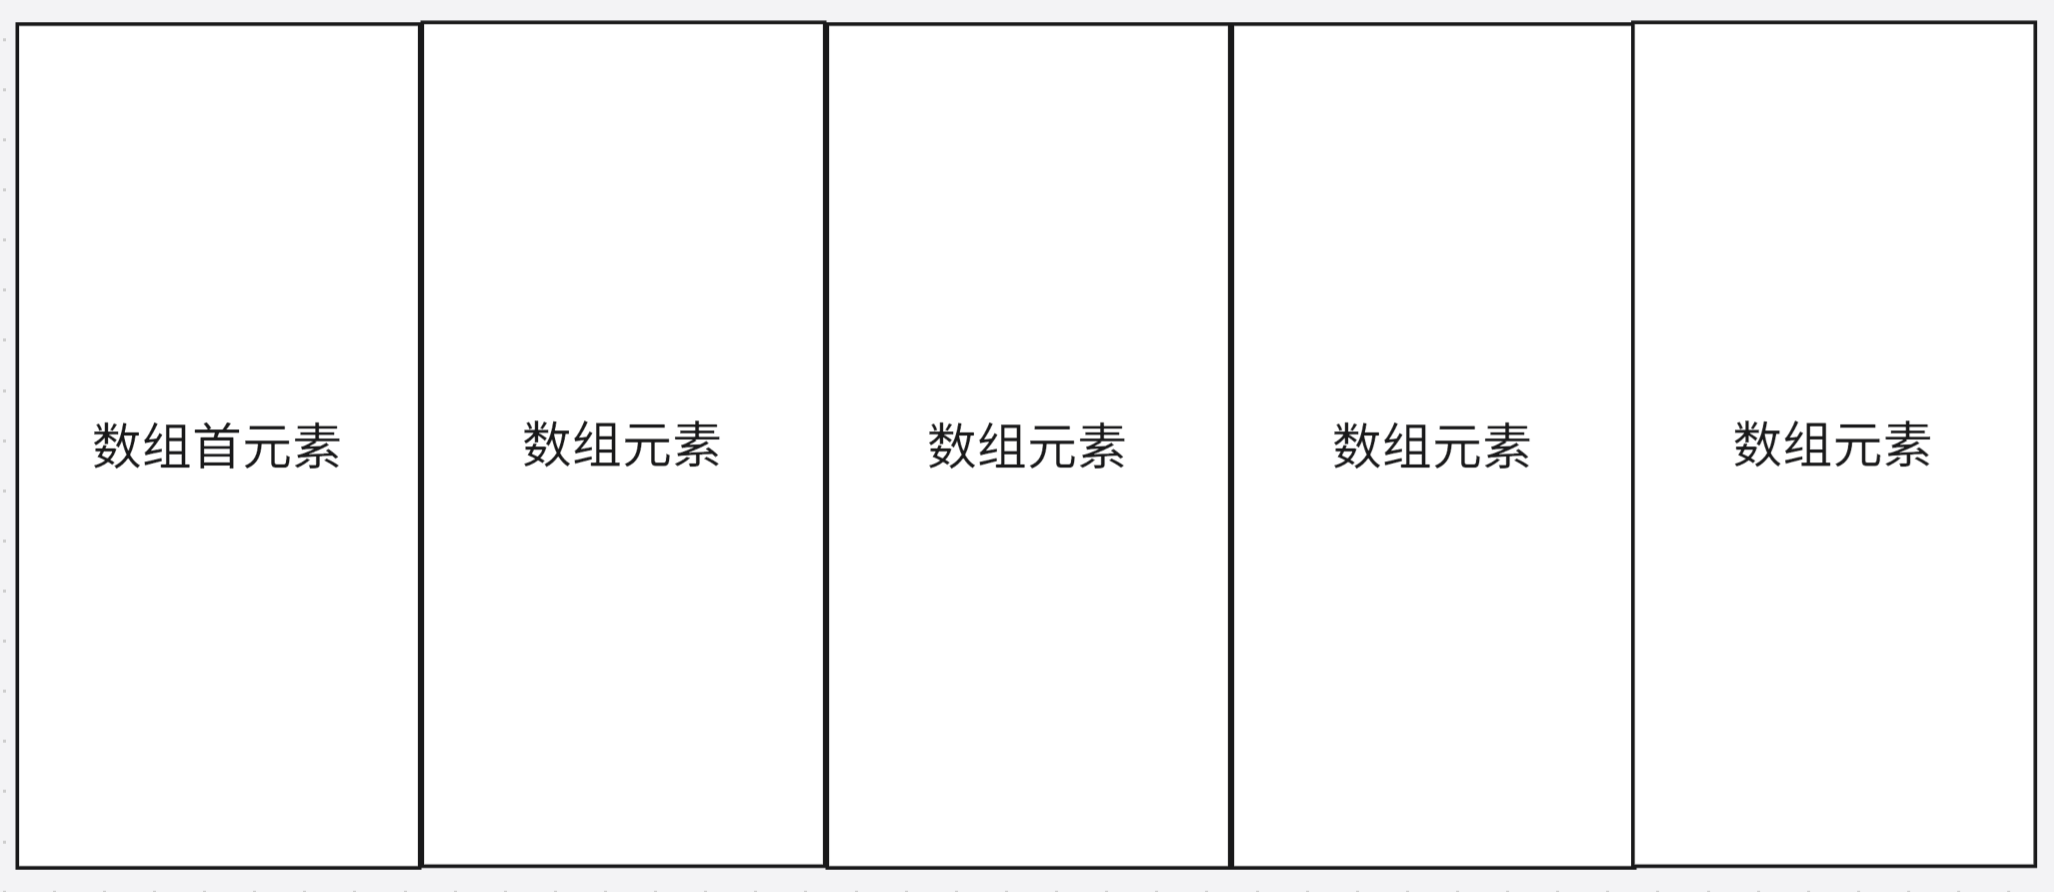
\includegraphics[width=0.7\textwidth]{数组.png}
    \caption{数组} % 图片标题
    \label{fig:数组} % 图片标签,用于引用
\end{figure}

\textbf{数组(Array)},又称\textbf{顺序表},它的STL容器有两种,分别是$array$和$vector$。

$array$是固定大小的数组。$vector$是一种动态数组,可以动态增长,可以根据需要自动分配内存。两者的声明方式如下:
\begin{tcode}
std::array<int,5> arr;
std::vector<int> vec;
\end{tcode}

$array$并不常用,因为它是固定大小的,如果需要改变大小,只能重新声明一个新的数组。
可以参考这篇blog详细了解:

\url{https://blog.csdn.net/qq_38410730/article/details/102802239}

$vector$由于其动态性,可以根据需要自动分配内存,因此使用起来比较方便,在工程实践中也更常用。
$vector$的实现原理是当检测到$vector$的容量不足时,会自动分配新的内存(原来的大小$\times$2),并将原有数据复制到新内存中。
这个复制的过程非常缓慢,因此,在使用大型的资源时,$vector$的效率可能会比较低。

成员函数(常用部分):
\begin{tcode}
std::vector<int> vec{1,2,3,4,5,6};
vec[0];         //访问(快速)
vec.at(0);    //访问(安全)
vec.front();    //第一个元素
vec.back();     //最后一个元素
vec.empty();    //检查是否为空
vec.size();     //返回容器大小
vec.reserve(10);//预留空间
vec.clear();    //清除所有元素
vec.insert(vec.begin(),1);//插入元素
vec.erase(vec.begin());//删除元素
vec.push_back(1); //在最后添加
vec.emplace_back(); //在最后添加
vec.pop_back();     //删除最后一个
\end{tcode}

\textbf{链表(List)}:链表是一种非连续的内存块,它是由一系列节点组成,每个节点都包含数据和指针。
链表的实现原理是每个节点都包含一个指针,指向下一个节点。链表的头节点称为头指针,尾节点称为尾指针。
链表的插入、删除操作都比较容易,只需要改变指针即可,但是查找操作比较麻烦,需要从头节点开始遍历。
\begin{figure}[H]
    \centering
    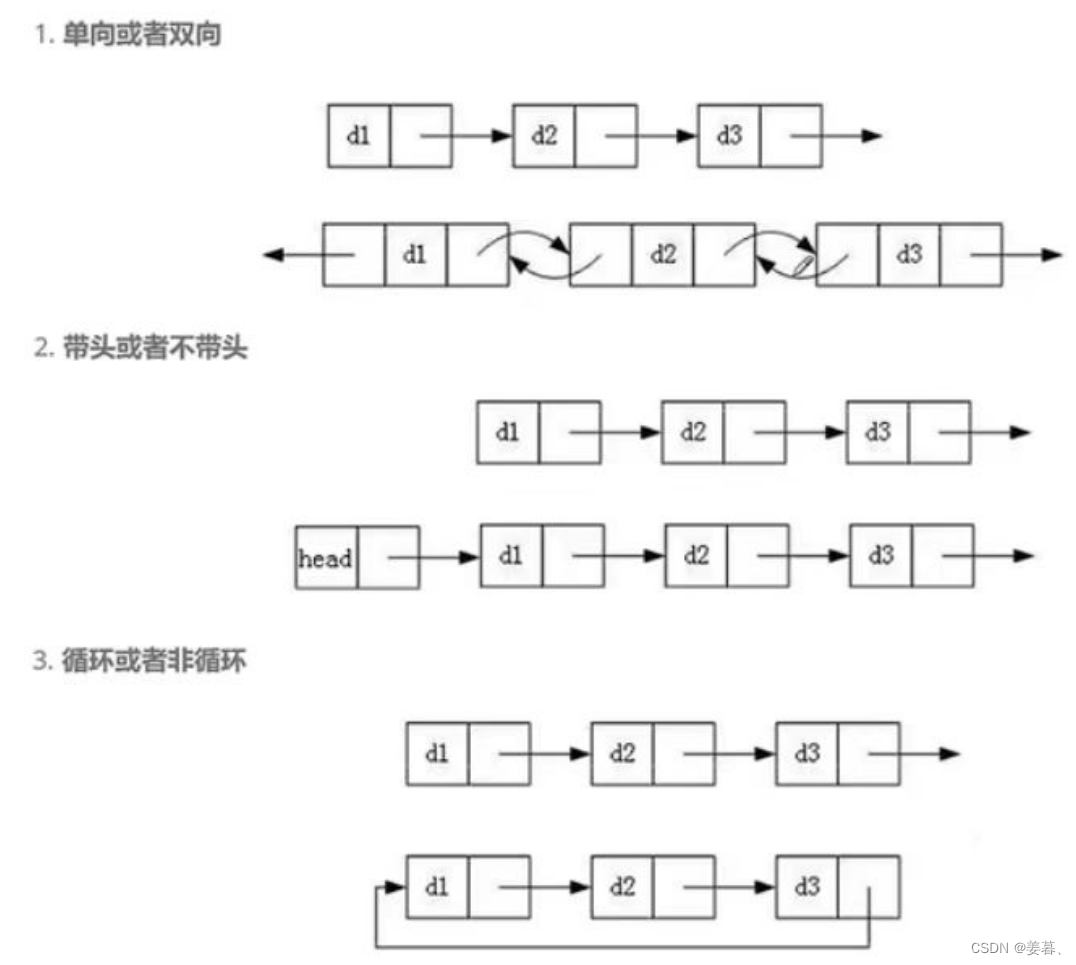
\includegraphics[width=0.7\textwidth]{链表1.png}
    \caption{链表} % 图片标题
    \label{fig:链表} % 图片标签,用于引用
\end{figure}

它的STL容器是$list$(双向链表)和$forward\_list$(单向链表)。比较简单,请自行去查阅相关文档:

\url{https://zh.cppreference.com/w/cpp/container/list}

\textbf{队列(Queue)}:队列是一种线性数据结构,它按照\textbf{先进先出}的原则进行操作。队列有两个基本操作,分别是\textbf{入队}和\textbf{出队}。入队操作是在队列的末尾添加一个元素,而出队操作是从队列的头部移除一个元素。队列有两个端点,队头和队尾,队头是队列的第一个元素,出队操作发生的地方,队尾是队列的最后一个元素,入队操作发生的地方。通常情况下,\textbf{不允许随机访问}队列中的元素,只能访问队头元素。
队列在\textbf{多任务处理、打印任务管理、缓冲处理}等场景中有广泛应用,它帮助维持操作的顺序和流程控制。
(很常用)
\begin{figure}[H]
    \centering
    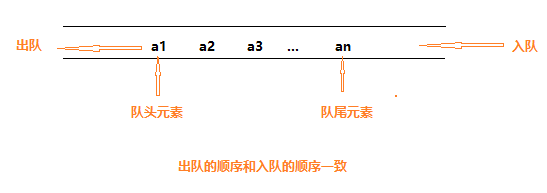
\includegraphics[width=0.7\textwidth]{队列1.png}
    \caption{入队和出队操作} % 图片标题
    \label{fig:入队和出队操作} % 图片标签,用于引用
\end{figure}
\begin{figure}[H]
    \centering
    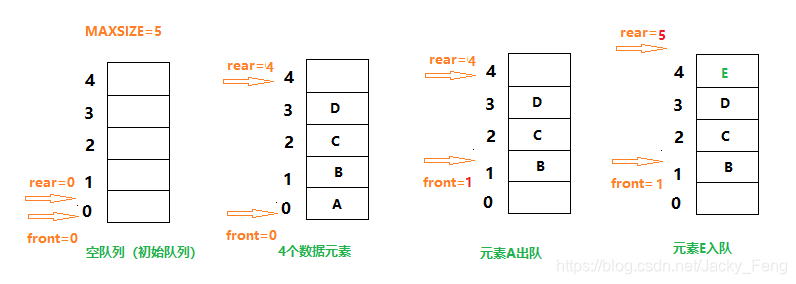
\includegraphics[width=0.7\textwidth]{队列2.png}
    \caption{队列实现方式} % 图片标题
    \label{fig:队列实现方式} % 图片标签,用于引用
\end{figure}

它的STL容器是$deque$,基于双向队列,C++还实现了3种容器适配器:
$stack$(堆栈),$queue$(单向队列),$priority\_queue$(优先队列),相较于$deque$,我们更常用$queue$
进行队列操作。
具体用法,请自行查阅相关文档:

\url{https://zh.cppreference.com/w/cpp/container/deque}

\url{https://zh.cppreference.com/w/cpp/container/queue}

\textbf{优先队列(Priority Queue)}:优先队列是一种特殊的队列,它允许插队的出现,可以根据“重要性”对队中元素进行排序。
优先队列的实现原理是每个元素都有一个优先级,优先级越高,元素越容易被取出。
优先队列的应用场景有很多,如任务调度、排序、搜索等。

\begin{figure}[H]
    \centering
    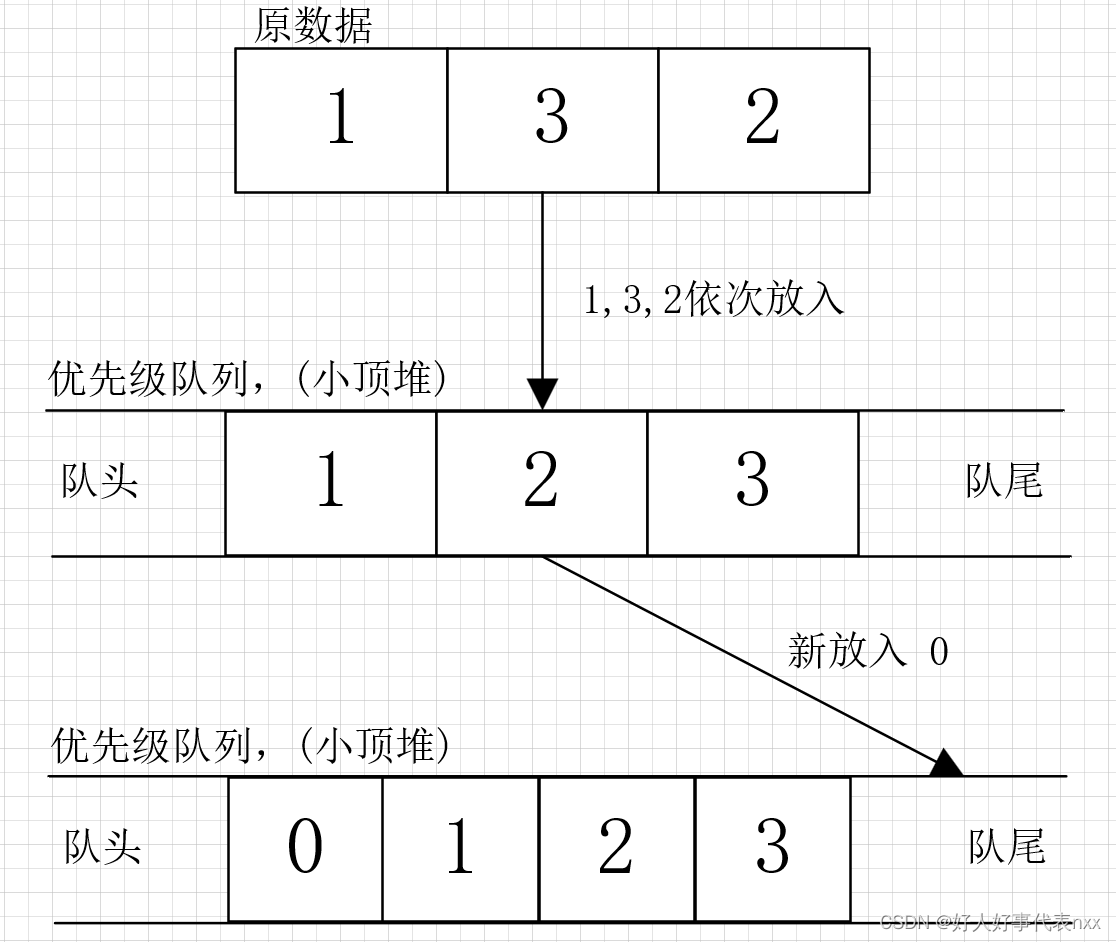
\includegraphics[width=0.7\textwidth]{优先队列1.png}
    \caption{优先队列} % 图片标题
    \label{fig:优先队列} % 图片标签,用于引用
\end{figure}

它的实现是容器适配器$priority\_queue$,
具体用法,请自行查阅相关文档:

\url{https://zh.cppreference.com/w/cpp/container/priority_queue}


\textbf{堆栈(Stack)}:堆栈是一种线性数据结构,它按照\textbf{先进后出}的原则进行操作。堆栈有两个基本操作,分别是\textbf{压栈}和\textbf{弹栈}。压栈操作是在堆栈的顶部添加一个元素,而弹栈操作是从堆栈的顶部移除一个元素。堆栈有两个端点,栈顶和栈底,栈顶是堆栈的顶部,压栈操作发生的地方,栈底是堆栈的底部,弹栈操作发生的地方。
堆栈在\textbf{函数调用、表达式求值、回溯、计算器、括号匹配、迷宫寻路}等场景中有广泛应用。

\begin{figure}[H]
    \centering
    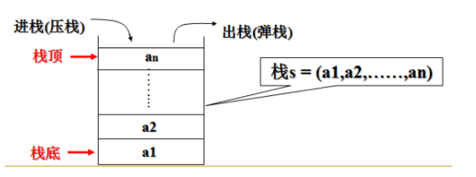
\includegraphics[width=0.7\textwidth]{堆栈1.png}
    \caption{压栈和弹栈操作} % 图片标题
    \label{fig:入队和出队操作} % 图片标签,用于引用
\end{figure}
\begin{figure}[H]
    \centering
    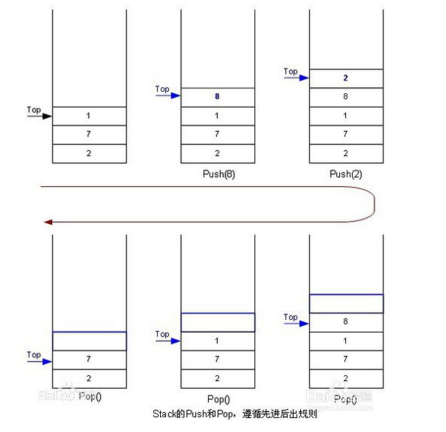
\includegraphics[width=0.7\textwidth]{堆栈2.png}
    \caption{堆栈实现方式} % 图片标题
    \label{fig:队列实现方式} % 图片标签,用于引用
\end{figure}

它的实现是容器适配器$stack$,
具体用法,请自行查阅相关文档。
\url{https://zh.cppreference.com/w/cpp/container/stack}

\textbf{树(Tree)}:树是一种非线性数据结构,它是由节点和边组成,节点之间存在着一种特定的关系。树的种类很多,如二叉树、二叉搜索树、AVL树、红黑树、B树、B+树、B*树等。
\begin{figure}[H]
    \centering
    \includegraphics[width=0.7\textwidth]{树1.png}
    \caption{树的逻辑图(了解即可)} % 图片标题
    \label{fig:队列实现方式} % 图片标签,用于引用
\end{figure}

\begin{figure}[H]
    \centering
    \includegraphics[width=0.7\textwidth]{树2.png}
    \caption{树的示意图} % 图片标题
    \label{fig:队列实现方式} % 图片标签,用于引用
\end{figure}

\textbf{堆(Heap)}:堆是一种特殊的树,它是一个\textbf{完全二叉树},即除叶节点外,其他的每个节点都有两个子节点。
每个节点都有一个值,并且每个节点\textbf{都大于或等于其子节点}(这是最大堆max-heap,类似的,还有最小堆min-heap)。堆的应用场景有很多,如排序、优先队列、图算法、堆排序等。

\begin{figure}[H]
    \centering
    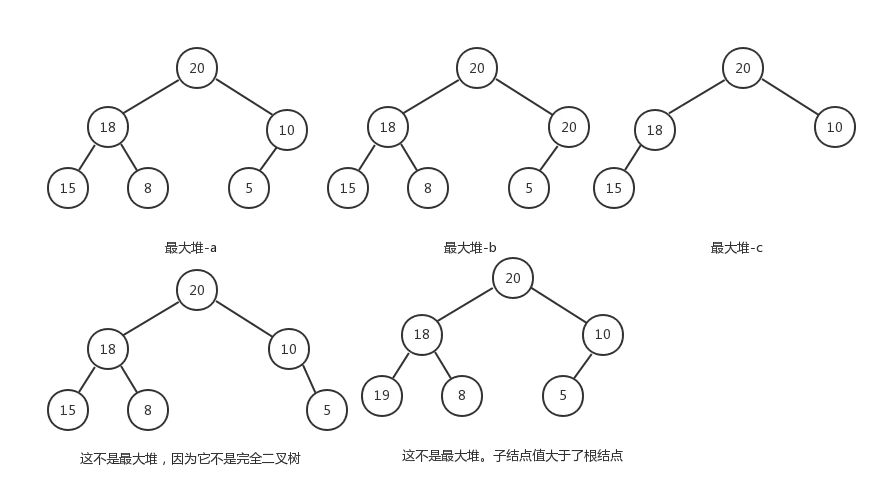
\includegraphics[width=0.7\textwidth]{最大堆.png}
    \caption{最大堆的示意图} % 图片标题
    \label{fig:最大堆} % 图片标签,用于引用
\end{figure}

\begin{figure}[H]
    \centering
    \includegraphics[width=0.7\textwidth]{堆1.png}
    \caption{最大堆和最小堆} % 图片标题
    \label{fig:最大堆和最小堆} % 图片标签,用于引用
\end{figure}

优先队列就是根据这个原理实现的,它是一种特殊的堆,具有\textbf{快速查找}的特性。他通过对于每个任务的重要程度进行编号,并将编号大的任务放在堆的顶部,这样就可以快速的找到重要的任务。
由于堆的排序算法非常快,可以实现更快速的任务调整,因此优先队列被广泛地应用于\textbf{任务管理}中。

优先队列的STL容器是$priority\_queue$。

具体用法,请自行查阅相关文档:

\url{https://zh.cppreference.com/w/cpp/container/priority_queue}

\textbf{映射(Map)}:映射是一种关联容器,它是一个\textbf{键值对}的集合,其中每个键都是唯一的,值可以重复。
映射的实现原理是通过哈希表(或红黑树)实现的,因此,查找、插入、删除操作的时间复杂度都是$O(1)$(或$O(logN)$)。

\textbf{红黑树(Red-Black Tree)}是一种随机查找速度比较快的\textbf{平衡二叉树}\footnote{
    平衡二叉树,也叫AVL树,它或者是一颗空树,或者具有以下性质的二叉排序树:它的左子树和左子树的高度之差(平衡因子)的绝对值不超过1,且它的左子树和右子树都是一颗平衡二叉树}
,他的查找、插入、删除操作的时间复杂度都是$O(logN)$ \footnote{
    O(logN)表示时间复杂度,N是问题的规模,O表示运行消耗时间的上界
}。

\textbf{哈希表(HashTable)}是一种\textbf{散列表},它通过\textbf{哈希函数}将键映射到值。
由于其使用计算来查找,因此,查找操作的时间复杂度都是$O(1)$
\footnote{常数的时间复杂度意味着不管问题的规模如何,
对于同一个长度的HashTable,算法的运行时间都不会随着问题的规模增加而增长。}。
但是哈希表的建立比较困难,需要消耗很多资源。
而且存储长度有限,当元素过多时,哈希表的性能会下降。当哈希表满时,需要执行\textbf{再散列(Rehashing)},解决\textbf{哈希冲突(Hash Collision)}问题,
这个过程需要消耗大量时间。

两者各有优劣,在实际应用中,需要根据具体问题选择。
红黑树型映射的STL容器是$map$,哈希表型映射的STL容器是$unordered\_map$,
具体用法,请自行查阅相关文档:

\url{https://zh.cppreference.com/w/cpp/container/map}

\subsubsection{STL的迭代器}

\textbf{迭代器},是一种检查容器内元素并遍历元素的数据类型,通常用于对C++中各种容器内元素的访问,
但不同的容器有不同的迭代器,初学者可以将迭代器理解为一个可以\textbf{自动向后移动的指针}。

常用的可迭代的容器有:

\begin{enumerate}
    \item 序列容器:$array$、$vector$、$deque$、$list$、$forward\_list$等
    \item 关联容器:$set$、$map$、$multimap$等
\end{enumerate}

$queue$、$stack$、$priority\_queue$是容器适配器,必须满足一定规则,没有迭代器。

对于可迭代容器,一般可以使用.begin()和.end()方法获取迭代器,.begin()方法返回指向第一个元素的迭代器,
.end()方法返回指向最\textbf{后一个元素的迭代器的下一位置}。
使用迭代器,可以方便的对容器内元素进行遍历,例如:

\begin{tcode}
std::vector<int> vec{1,2,3,4,5,6,7,8,9,0};
for(auto it = vec.begin();it != vec.end();++it){
    std::cout << *it << std::endl;
}
\end{tcode}

也可以简写为:

\begin{tcode}
for (auto it: vec) {
    std::cout << it << std::endl;
}
\end{tcode}

还可以使用迭代器对容器内元素进行修改,例如:

\begin{tcode}
std::vector<int> vec{1, 2, 3, 4, 5, 6, 7, 8, 9, 0};
vec.erase(vec.begin()+5);//删除第6个元素
vec.erase(vec.begin()+5,vec.end());//删除第6个元素之后的所有

std::vector<int> vec1{1, 2, 3, 4, 5, 6, 7, 8, 9, 0};
std::iter_swap(vec1.begin(),vec1.begin()+1);//交换第一个和第二个元素

std::vector<int> vec2{1, 2, 3, 4, 5, 6, 7, 8, 9, 0};
//此函数需要头文件<algorithm>
std::sort(vec2.begin(),vec2.end(),[](int& a,int& b){
    return a>=b;
});

//此函数需要头文件<algorithm>
//删除大于5的元素
auto newVec = std::remove_if(vec2.begin(),vec2.end(),[](int& a){
    return a>5;
});
\end{tcode}

我们不会使用十分复杂的迭代器,感兴趣的同学可以看一下cppreference的相关文档:

\url{https://zh.cppreference.com/w/cpp/iterator}

\textbf{迭代器失效}:迭代器失效指的是迭代器因为某些操作而不再指向原来的元素,
或者不再保持有效的状态,这样的迭代器如果继续使用,可能会导致未定义行为,包括程序崩溃。
通俗的理解就是,当你对容器进行了操作时,更改了容器的大小,但是迭代器仍然指向原来的位置,
这样就会导致读取错误的内存,这就是迭代器失效。

\begin{tcode}
std::vector<int> vec={1,2,3,4,5,6,7,8,9,10};
for(auto it = vec.begin(); it!= vec.end(); ++it){
    if(*it%2==0){
        vec.erase(it);
    }
}
\end{tcode}

看上面的代码,当执行到vec.erase(it)时,it已经失效,因为执行了erase之后,
vec的大小发生了变化,这导致了迭代器失效。

在实践过程中, 在下面的几种情况下,迭代器会失效,需要\textbf{避免}出现:
\begin{enumerate}
    \item 当执行erase方法时,指向删除节点的迭代器全部失效,指向删除节点之后的全部迭代器也失效
    \item 当进行push\_back\(\)方法时,end操作返回的迭代器肯定失效。
    \item 当插入\(push_back\)一个元素后,capacity返回值与没有插入元素之前相比有改变,
    则需要重新加载整个容器,此时first和end操作返回的迭代器都会失效。
    \item 当插入\(push_back\)一个元素后,如果空间未重新分配,指向插入位置之前的元素的迭代器仍然有效,但指向插入位置之后元素的迭代器全部失效。
\end{enumerate}

对于关联容器,使用迭代器时,删除一个键值对知识当前这个迭代器失效,别的迭代器不会受到影响,
这可能是由于底层使用红黑树实现的原因,但是实际应用中,仍然不应该冒这个风险,因此,
必须\textbf{坚决避免迭代器失效问题的发生}。

在具体的应用中,我们在使用迭代器遍历时,应该注意不要对容器进行增删操作,更不应该改变容器的大小。
可以将不需要的元素放在\textbf{容器的末尾}或者\textbf{记录下需要删除的迭代器},然后适时删除。例如:

\begin{tcode}
for(auto it = vec.begin(); it!= vec.end(); ++it){
    if((*it)%2==0){
        its.push_back(it-vec.begin());
    }
}

int i=0;
for(auto it : its){
    vec.erase(vec.begin()+it-i);
    i++;
}
}
\end{tcode}

这种方法,非常\textbf{不优雅},因此,\textbf{不要使用}。

\textbf{更多的用法等待着同学们自己去探索!}

\subsubsection{系统级内存运行逻辑}

C++是一个十分灵活的编程语言,其中指针的概念为程序员们提供了直接操纵内存的能力。
指针的使用使得程序员可以自由的操作内存,但是也带来了一些安全性和复杂性问题。
因此,了解程序运行的底层逻辑,对于理解C++至关重要,对于提高程序效率举重若轻,下面我们来看看C++的内存运行逻辑。

\begin{figure}[H]
    \centering
    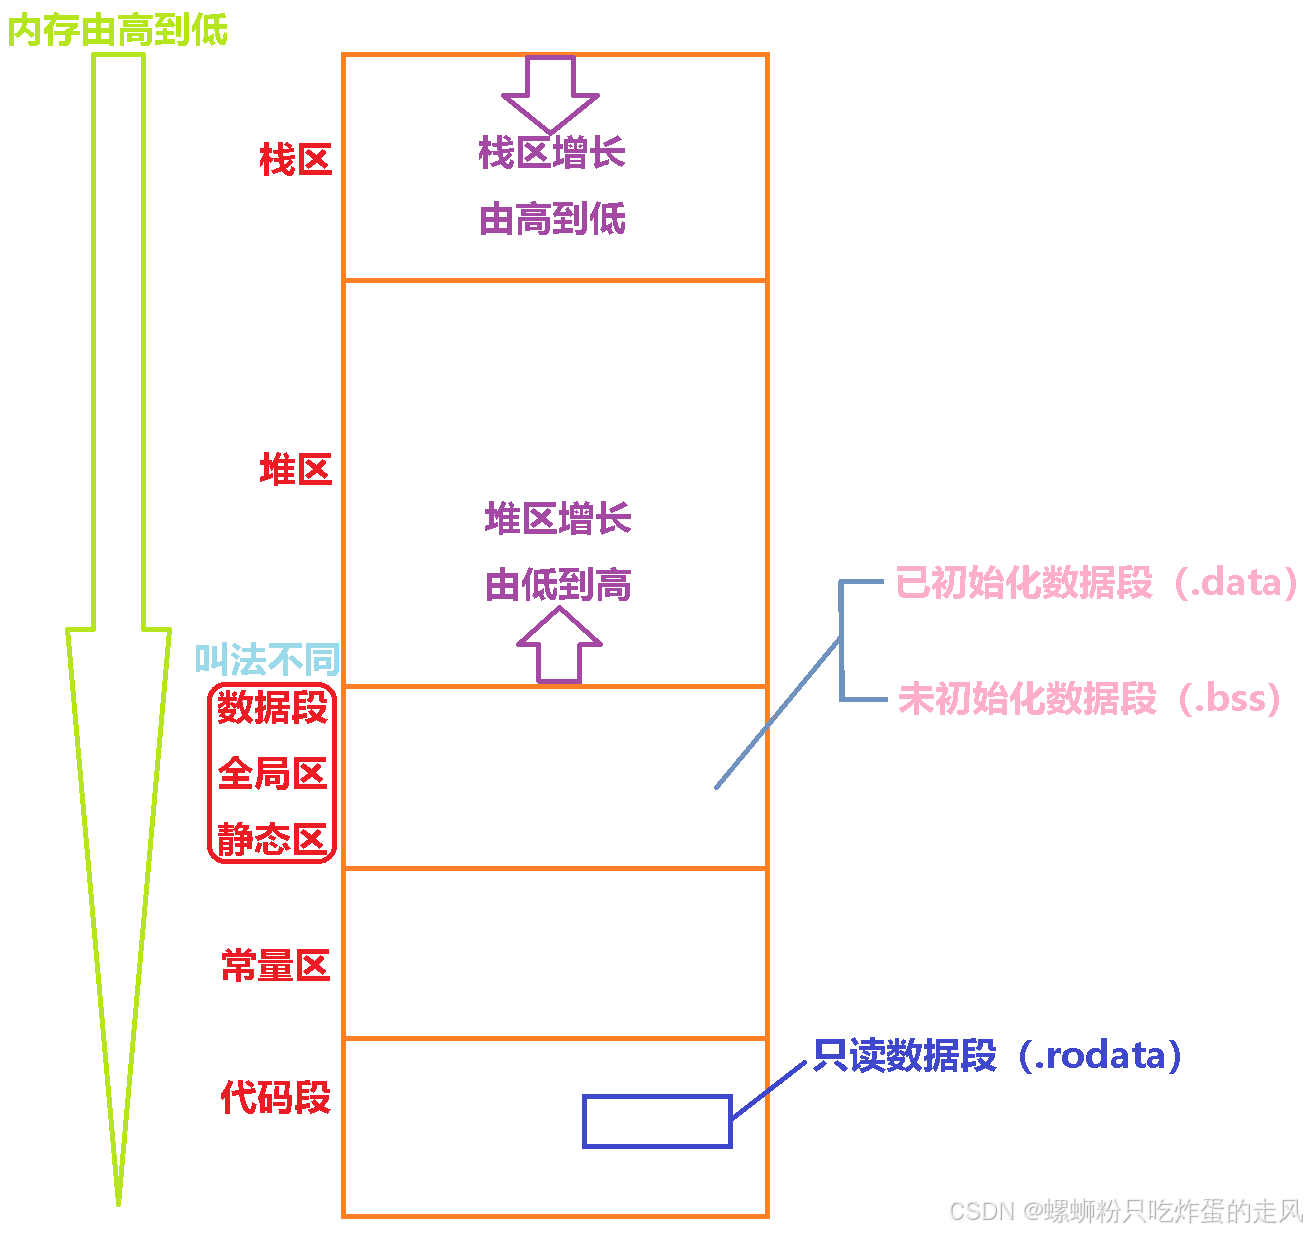
\includegraphics[width=0.7\textwidth]{系统内存.png}
    \caption{系统内存分区} % 图片标题
    \label{fig:内存分区} % 图片标签,用于引用
\end{figure}

如图\ref{fig:内存分区},系统内存分为\textbf{代码区、常量区、全局/静态变量区、堆区、栈区等几个部分}。

\textbf{代码区和常量区}是存放程序代码和常量数据的区间一般不作区分,这里的数据是只读的,其中存储着一些在编译过程前就可以确定的数据内容
,如代码、$constexpr$修饰的变量、$const$修饰的在预编译期可以确定的值等,
一些字面常量如"Hello World!",也存储于其中。程序在常量区中只能读取数据。

\textbf{全局/静态变量区}是存放全局/静态变量的区间,全局变量在程序运行前就已经分配了内存,静态变量在程序运行前也已经分配了内存。
但是静态变量的生命周期比全局变量长,它在程序运行结束后才释放内存。

\begin{enumerate}
    \item 全局变量:在函数外部定义的变量,它们具有全局作用域。
    \item 静态全局变量:在函数外部定义并用 $static$ 关键字修饰的变量,它们具有内部链接属性,即它们只能在定义它们的文件内部可见。
    \item 静态局部变量:在函数内部定义并用 $static$ 关键字修饰的变量,它们在函数调用结束后仍然存在,并且保持它们的值。
    \item 类静态成员变量:在类定义中使用 $static$ 关键字声明的成员变量,它们属于类而不是类的任何一个实例。
\end{enumerate}

解释一下\textbf{静态}:
\begin{enumerate}
    \item 生命周期上,静态变量在程序开始运行前或类的实例化之前就已经分配了内存,在程序运行结束后才释放内存。地址不会发生变化,就静静“躺”在静态变量区,直到程序结束。
    \item 相对于$new$的动态分配,可以让程序员选择什么时候分配和释放内存,而$static$变量则是一直存在的,直到程序结束。
    \item 静态全局变量也具有全局作用域,他与全局变量的区别在于如果程序包含多个文件的话,他作用于定义它的文件里,不能作用到其他文件里,即被$static$关键字修饰过的变量具有文件作用域。这样即使两个不同的源文件都定义了相同的静态全局变量,他们也是不同的变量。这点于全局变量不同。
\end{enumerate}

\textbf{堆区}:堆区是由程序员手动分配和释放的内存,堆区的分配和释放由\textbf{程序员控制},程序员可以通过$new$和$delete$操作符来分配和释放内存。

在大小上,堆区的大小相对于栈区是很大的,因此可以存储更多的数据。初次之外,堆区是由程序员全权负责管理的,程序员必须小心管理堆区的分配和释放,确保程序的正确性和安全性,一般使用\textbf{智能指针}和$nullptr$判断提高程序的稳定性。
但与此同时,堆区也提供了更为灵活的编程和数据传递模式,可以参考下面的例子:
\begin{tcode}
std::vector<int>* func(){
    std::vector<int>* a = new std::vector<int>({1,2,3,4});
    std::vector<int> b{1,2,3,4};
    return a;//return &b;
    //换成return &b;之后再试试呢?
}

int main() {
    auto vecPtr = func();
    return 0;
}
\end{tcode}

\textbf{栈区}:栈区是由\textbf{编译器自动分配和释放的内存},栈区的分配和释放都是编译器\textbf{自动完成}的,程序员\textbf{无法直接控制}栈区的分配和释放。
栈区存储数据的优势在于\textbf{快速},但是也有一些缺点,比如栈区的大小是有限的,因此在函数调用层次过深时,可能会出现栈溢出。
栈区的大小一般是$2MB$,因此栈区的大小是有限制的,如果函数调用层次过深,可能会出现栈溢出。

\textbf{系统内存管理}:系统内存管理是操作系统的工作,它负责分配和释放系统内存,其中操作系统会自行决定栈内存,下面我们讨论一下栈区的操作。

在栈内存中,数据存储在系统栈中,只有一个开口,数据只能从栈顶入栈和出栈。在切换代码的\textbf{作用域}时,上一个作用域的数据会被新的数据压在栈的下方,
这些数据将不能被当前的程序进程所读取,直到当前的这些数据被弹出栈。
栈内存的设计是十分精妙的,它可以有效的解决内存分配和释放的问题,亦可以实现函数的层次调用,作为一名C++程序员,我们要理解透彻栈内存的运行逻辑。

\textbf{函数递归的底层原理}:函数递归是一种非常有趣的编程技巧,它可以让程序员以一种\textbf{迭代}的思想来理解和编写代码。

\begin{figure}[H]
    \centering
    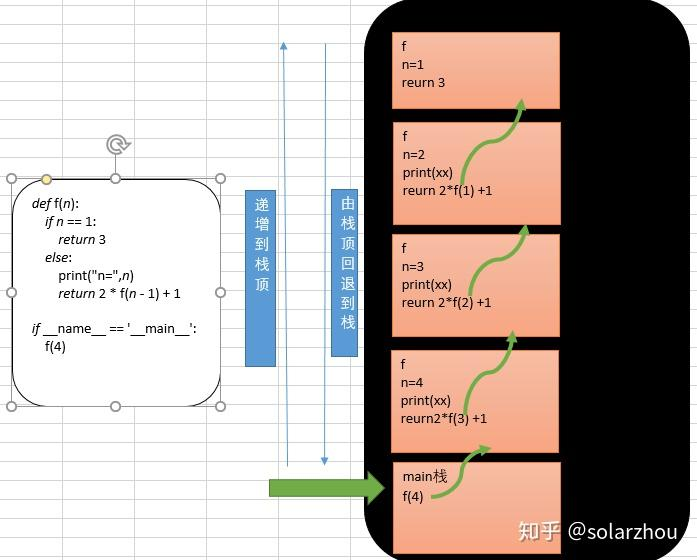
\includegraphics[width=0.7\textwidth]{栈递归.jpg}
    \caption{函数递归调用栈} % 图片标题
    \label{fig:栈递归} % 图片标签,用于引用
\end{figure}

在函数调用时,新的函数的栈帧会被压入栈中(称为栈帧),从而覆盖掉原来的\textbf{栈帧},当函数返回时,栈帧会被弹出栈。
露出原来的函数栈帧。当函数调用自身时,会形成一个\textbf{递归调用栈}。

需要注意的是,栈内存的大小是有限制的,当函数调用层次过深时,会出现栈溢出。

\subsubsection{C++的多线程}

多线程技术是C++中非常重要的特性之一,它可以让程序员以更高的并发性和速度运行程序。使用多线程可以提高程序的运行效率,丰富程序的运行逻辑,实现许多单线程所不能实现的功能。
在C++中,提供了$<threaed>$库来实现多线程的功能。

\textbf{多线程的原理}:多线程是指在同一程序中同时运行多个线程来完成不同的任务,以提高资源利用率和程序响应速度。
硬件条件上,多线程需要CPU支持多核处理或多任务处理,以及足够的内存和处理器资源。在多线程编程过程中,可能遇到一些问题,
包括线程同步、死锁、竞态条件等,这些问题可能导致程序运行不稳定、性能下降甚至系统崩溃。
因此,在设计多线程程序时,需要充分考虑线程之间的\textbf{协作与互斥},合理分配资源,以保障程序的正确性和高效性。
在多线程之中,有两种主要的设计模式,即\textbf{阻塞}和\textbf{非阻塞}。

\begin{enumerate}
    \item \textbf{阻塞}:在阻塞模式下,线程在等待某个事件的发生,如等待IO操作完成、等待子进程结束等。
当某个事件发生时,线程会被唤醒,并开始执行。

    \item \textbf{非阻塞}:在非阻塞模式下,线程在等待某个事件的发生,但不会被挂起,而是继续执行后续代码。
当某个事件发生时,线程会被通知,并开始执行。
\end{enumerate}


\textbf{创建线程}:
C++11中引入的$<thread>$库提供了多线程的支持,它提供了$std::thread$类来创建和管理线程:

\begin{tcode}
用法:std::thread ThreadName(函数指针,[参数]);
实例:
void function1(){for(int i=0;i<1000;i++);}
void function2(int a,int &b){for(int i=0;i<1000;i++);}
int main() {
    std::thread th1(function1);
    int a=0, b=0;
    std::thread th1(function1,a,std::ref(b));
    return 0;
}
\end{tcode}

如果你想要在线程中传递参数,可以直接传递参数,也可以使用引用传递参数,引用传参的时候需要使用$std::ref()$函数。
你也可以使用$join()$方法使主线程等待所有线程结束,
$detach()$方法将线程分离,这样主线程就不会等待主线程结束而结束。

\textbf{线程同步和互斥锁}:
多线程程序的稳定性和互斥锁是多线程编程中经常遇到的问题。请参考下面的例子:
\begin{tcode}
int i=0;
void function1(){
    for(int j=0;j<100000;j++)
        i++;
}

int main() {
    std::thread th1(function1);
    for(int j=0;j<100000;j++)
        i++;
    if(th1.joinable())
        th1.join();
    std::cout << i;
    return 0;
}
\end{tcode}
在程序的运行过程中,$i$的值可能是$0$,也可能是$200000$,这取决于线程的调度。
当两个线程同时拿到$i$的地址时,同时对i进行写入操作,两者就会出现线程同步问题。
那怎么解决这个问题呢?$std::mutex$和$std::lock\_guard$为我们提供了解决方案——互斥锁。是解决线程同步问题的两种方法。
$mutex$是一种同步机制,它可以保证同一时刻只有一个线程对共享资源进行访问。
$lock\_guard$是一个智能指针,它可以自动获取互斥锁,并在离开作用域时自动释放互斥锁。

\begin{tcode}
#include <iostream>
#include <thread>
#include <mutex>

int i=0;
std::mutex lock;
void function1(){
    for(int j=0;j<100000;j++){
        lock.lock();
        i++;
        lock.unlock();
    }
}

int main() {
    std::thread th1(function1);
    for(int j=0;j<100000;j++){
        lock.lock();
        i++;
        lock.unlock();
    }
    if(th1.joinable())
        th1.join();
    std::cout << i;
    return 0;
}
\end{tcode}
发现程序的稳定性已经得到提高,在多次运行过程中,$i$的值始终是$200000$。这一点在多线程编程过程中非常重要,是所有程序员的必修课。
但是,这是又产生了一个新的问题,那就是程序员还是需要进行互斥锁的手动管理,这无疑会降低程序开发的效率。
类似于智能指针的,C++11中引入了$std::lock\_guard$来自动管理互斥锁,它可以自动获取互斥锁,并在离开作用域时自动释放互斥锁。

\begin{tcode}
#include <iostream>
#include <thread>
#include <mutex>

int i=0;
std::mutex lock;
void function1(){
    for(int j=0;j<100000;j++){
        std::unique_lock<std::mutex> Autolock;
        i++;
    }

}

int main() {
    std::thread th1(function1);
    for(int j=0;j<100000;j++){
        std::unique_lock<std::mutex> Autolock;
        i++;
    }

    if(th1.joinable())
        th1.join();
    std::cout << i;
    return 0;
}
\end{tcode}
程序测试成功,$i$的值始终是$200000$。

\textbf{死锁}:在使用互斥锁的时候,如果多个线程都在\textbf{等待对方释放锁},就会出现死锁。请看下面的例子:

\begin{tcode}
int i=0;
std::mutex lock1;
std::mutex lock2;
void function1(){
    for(int j=0;j<100000;j++){
        lock1.lock();
        lock2.lock();
        i++;
        lock2.unlock();
        lock1.unlock();
    }
}

int main() {
    std::thread th1(function1);
    for(int j=0;j<100000;j++){
        lock2.lock();
        lock1.lock();
        i++;
        lock2.unlock();
        lock1.unlock();
    }

    if(th1.joinable())
        th1.join();
    std::cout << i;
    return 0;
}

\end{tcode}

在这个例子中,两个线程都在等待对方释放锁,导致死锁。在设计时,尽量使得不同的互斥锁以相同的顺序被获取和释放,可以降低死锁的概率。

\textbf{原子变量}:在C++11中,引入了原子类型$std::atomic$,它可以保证变量的原子性,即在读写操作时,其他线程只能看到该变量的\textbf{已修改}值。
使用这种方式,可以增强程序的可读性。原子变量也不需要使用互斥锁进行同步,它可以自动保证原子性。

\textbf{条件变量}:条件变量($Condition Variable$)是一种用于线程同步的机制,通常与互斥锁($Mutex$)一起使用。条件变量提供了一种线程间的通信机制,允许一个线程等待另一个线程满足某个条件后再继续执行。

我们通过一个例子来简单理解一下这个问题:

现在小明在一张桌子上放一个苹果,而旁边有一群蒙着眼睛的人,因为他们的眼睛被蒙着,
他们如果想拿到这个苹果,就会时不时来桌子前摸一摸看看桌子是否有苹果,并且谁来桌子前摸苹果是无序的,
这时的场面就很混乱,小明一看不行,于是小明就桌子上放了个铃铛,并且组织需要苹果的人排好队,
有苹果小明就会摇响铃铛,排在第一个的人就拿走苹果,然后如果还想要苹果就到队尾排队等待
。此时混乱的场面就显得井然有序了。在本故事中,小明就是操作系统,苹果就是临界资源,
一群蒙着眼睛都人就是多线程,铃铛就是条件变量,排队就是实现同步,摇响铃铛就是唤醒线程。

使用条件变量主要是因为它们提供了在多线程编程中一种有效的同步机制。
当多个线程需要\textbf{等待某个特定条件}成立才能继续执行时,条件变量就显得尤为重要。
通过条件变量,线程可以安全地进入等待状态,直到被其他线程显式地唤醒或满足等待的条件。
这有助于避免线程的\textbf{无谓轮询或忙等待},提高了系统的响应能力和效率。
\textbf{注意}:在使用条件变量时,必须确保与\textbf{互斥锁}一起使用,以\textbf{避免竞态条件}的发生。

下面介绍一下$condition\_variable$的用法:

调价变量的使用大致可以分为两个大的功能,即$notify$和$wait$。

\begin{tcode}
std::condition_variable condition;//声明
condition.notify_all();//通知所有等待线程
condition.notify_one();//通知第一个接收的等待线程

std::unique_lock<std::mutex> Lock(mtx);
condition.wait(Lock);//等待条件成立
condition.wait(Lock,[](){return true;});//等待条件和第二个参数同时为true
\end{tcode}

\textbf{消费者-生产者模型},是多线程编程中经常使用的模型。
生产者-消费者模型是指多个生产者线程和多个消费者线程之间通过一个共享的缓冲区进行通信。
生产者线程负责生产数据,并将其放入缓冲区;消费者线程则负责从缓冲区中取出数据进行消费。
生产者和消费者之间通过一个\textbf{条件变量}进行同步,以保证缓冲区中的数据不会被消费者线程消费完。

\begin{tcode}
#include<iostream>
#include<thread>
#include<mutex>
#include<condition_variable>
#include<queue>
#include<functional>

std::mutex lock;
std::condition_variable cv;
std::queue<std::function<void()>> taskQueue;
void consumer(){
    while(1){
        std::unique_lock<std::mutex> Lock(lock);
        cv.wait(Lock,[&](){
            return !taskQueue.empty();
        });
        auto task = taskQueue.front();
        task();
        taskQueue.pop();
        Lock.unlock();
    }
}

void producer(int i){
    auto func = [](int id){
        std::cout << "task" << id << " is running!" << std::endl;
    };
    std::function<void()> task = std::bind(func,i);
    {
        std::unique_lock<std::mutex> Lock(lock);
        taskQueue.push(task);
    }
    cv.notify_one();
    std::this_thread::sleep_for(std::chrono::seconds(1));
}

int main(int argc,char** argv){
    std::thread consumer_thread(consumer);
    for(int i=0;i<100;i++){
        producer(i);
    }

    if(consumer_thread.joinable())
        consumer_thread.join();
    return 0;
}
\end{tcode}

\textbf{线程池}:线程池是一种常用的技术,它可以提高程序的并发性,减少线程创建和销毁的开销,并可以有效的利用系统资源。
下面是一种线程池的实现方式,尝试一下把它看懂吧!

\begin{tcode}
#include <iostream>
#include <thread>
#include <mutex>
#include <condition_variable>
#include <functional>
#include <vector>
#include <queue>

class ThreadPool
{
private:
    std::vector<std::thread> threads;
    std::queue<std::function<void()>> tasks;
    std::mutex mtx;
    std::condition_variable condition;
    bool stop;

public:
    ThreadPool(int numThreads):stop(false) {
        for (int i = 0; i < numThreads; i++) {
            threads.emplace_back([this] {
                while (1) {
                    std::unique_lock<std::mutex> lock(mtx);
                    condition.wait(lock, [this] {
                        return !threads.empty() || stop;
                    });
                    if (stop && tasks.empty())
                        return;

                    auto task = std::move(tasks.front());
                    tasks.pop();
                    lock.unlock();
                    task();
                }
            });
        }

    }

    ~ThreadPool() {
        {
            std::unique_lock<std::mutex> lock(mtx);
            stop = true;
        }
        condition.notify_all();
        for (auto& iter : threads) {
            iter.join();
        }
    }

    template<class F, class ...Args>
    void enqueue(F&& f, Args&&... args) {
        std::function<void()> task =
                std::bind(std::forward<F>(f), std::forward<Args>(args)...);
        {
            std::unique_lock<std::mutex> lock(mtx);
            tasks.emplace(std::move(task));
        }
        condition.notify_one();
    }

};

int main() {
    ThreadPool Pool(4);
    for (int i = 0; i < 100; i++) {
        Pool.enqueue([i] {
            std::cout << "task" << i << "is running!" << std::endl;
            std::this_thread::sleep_for(std::chrono::seconds(1));
            std::cout << "task" << i << "has finished!" << std::endl;
        });
    }

    return 0;
}
\end{tcode}

\section{编译原理与CMake基础}

在实际工程中,编译器的选择往往是影响编译速度的关键因素。CMake是一种跨平台的编译工具,它可以用来管理工程的构建,自动生成makefile或project文件,并提供方便的接口来调用编译器、链接器等工具。

\subsection{C++的编译过程}

C++的编译过程可以分为以下几个步骤:

\begin{enumerate}
    \item \textbf{预处理}(Preprocessing):预处理器会对源代码进行预处理,将所有的宏定义、条件编译等操作展开,生成一个新的源文件。
    \item \textbf{编译}(Compilation):编译器会将预处理后的源文件编译成汇编语言。
    \item \textbf{汇编}(Assemble):汇编器会将汇编语言代码转换成机器语言。
    \item \textbf{链接}(Linking):链接器会将多个目标文件和库文件链接成一个可执行文件。
\end{enumerate}

\begin{figure}[H]
    \centering
    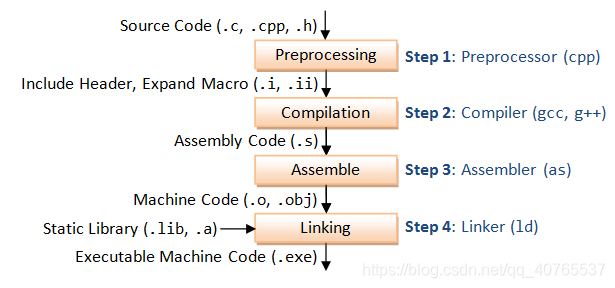
\includegraphics[width=0.7\textwidth]{编译流程.png}
    \caption{C++编译过程} % 图片标题
    \label{fig:编译} % 图片标签,用于引用
\end{figure}

\textbf{预编译}:
预编译器会对源代码进行预处理,将所有的宏定义、条件编译等操作展开,生成一个新的源文件。
预编译器的作用主要是对源代码进行预处理,以便于编译器进行编译。
比如说,对于一个头文件引用$\#include<iostream>$,预编译器会将其展开为头文件的源代码,
生成一个新的源文件,然后再进行编译。对于头文件,预编译器只会进行一次,而对于源文件,
预编译器会在每个源文件编译前进行一次。在代码中的宏定义$\#define$会在预编译时进行字符串替换,
而条件编译$\#if$则会根据条件是否成立来决定是否展开代码。
只有理解了这些,才能真正理解宏和条件编译的作用。

在C/C++中有一些预定义的宏,可以拿来直接用,如:
\begin{tcode}
__FUNTION__  获取当前函数名 
__LINE__ 获取当前代码行号 
__FILE__ 获取当前文件名 
__DATE__ 获取当前日期 
__TIME__ 获取当前时间
__STDC_VERSION__  获取当前编译器的版本
\end{tcode}

\textbf{编译}:
编译器会将预处理后的源文件编译成汇编语言。
编译阶段进行语法分析、词法分析和语义分析,并且将代码优化后产生相应的汇编代码文件(ASCLL文件),
即.s 文件。这个过程是整个程序构建的核心部分,也是最复杂的部分之一。

\textbf{汇编}:
通过不同平台(Windows、Linux)的汇编器将汇编代码翻译成机器码,即生成二进制可重定向文件(.o)。
任何一个源文件在进行编译阶段的时候会去产生\textbf{符号表},符号表中存放的就是程序所产生的符号
(例如:函数名,变量名等),我们的编译阶段是不会去给符号分配正确的地址。这些\textbf{符号}都没有被分配地址,
因此.o文件没有经过链接是无法执行的。

\textbf{链接}:
链接器会将多个目标文件和库文件链接成一个可执行文件。
链接器的作用是将多个目标文件和库文件链接成一个可执行文件,这个过程会将符号表中的符号分配正确的地址,
并将各个目标文件中的代码和数据合并到一个可执行文件中。
简单来说,\textbf{连接就是将符号和数据进行整合,最终得到一个可以指定的文件。}

链接有两种方式:\textbf{静态链接}和\textbf{动态链接}。
相对应的,这两种链接方式所对应的库就称为\textbf{静态库}和\textbf{动态库}。

\textbf{静态库}:
静态库是编译好的目标文件,在链接时会被直接链接到可执行文件中。
静态库的优点是编译速度快,缺点是可执行文件体积大,因为它包含了所有程序需要的目标文件。

\textbf{动态库}:
动态库是运行时加载的库,在程序运行时才被加载到内存中。
动态库的优点是可执行文件体积小,缺点是运行速度慢,因为它需要在运行时加载。

\subsection{CMake}
从上面的介绍中,可以看出,编译过程是十分复杂的,错误的编译方式可能会导致编译失败,或者编译的程序无法正确运行。
为了告诉编译器如何编译我们的程序,工程师们开发了$makefile$,它是一种描述编译过程的脚本文件。
$makefile$的优点是简单易懂,缺点是不够灵活,工程师需要写大量的$makefile$,并且需要手动管理。
在这种困境下,CMake应运而生。

\textbf{CMake}是一种跨平台的编译工具,它可以用来管理工程的构建,自动生成$makefile$或$project$文件,
并提供方便的接口来调用编译器、链接器等工具。$CMake$的优点是简单易用,它会根据工程的结构自动生成$makefile$,
并且可以自动检测编译器、库的安装路径,使得工程师只需要关注工程的源代码即可。

CMake的使用十分简单,只需要在工程的根目录下创建一个$CMakeLists.txt$文件,然后在其中写入编译指令即可。
主要的工作内容有:

\begin{enumerate}
    \item \textbf{项目配置}:确定工程的名称、版本、作者、编译器、编译器版本、编译类型等。
    \item \textbf{添加文件}:添加工程需要编译的源文件和头文件,查找依赖包,并将其加入编译列表。
    \item \textbf{编译}:使用CMake提供的接口编译工程,生成重定向文件和库文件。
    \item \textbf{连接}:将重定向文件和库文件链接成可执行文件。
    \item \textbf{安装}:将可执行文件安装到指定目录。
\end{enumerate}

下面我们来逐个分析介绍一下CMake的使用方法:

\subsubsection{项目配置}
使用CMake的第一步是配置工程,首先需要创建一个$CMakeLists.txt$。
在$CMakeLists.txt$文件中,
我们需要指定工程的信息,如项目名称、编译器、编译器版本、编译选项等。需要强调的是,
$CMake$本身\textbf{不具有编译功能},它只是用来管理工程的构建,具体来说,是形成一套编译器可以“看懂”的文件
然后编译器根据这些文件进行编译。

常用的命令有:
\begin{tpython}
project(project_name)  # 设置项目名称
cmake_minimum_required(VERSION 2.8)  # 设置CMake的最低版本
set(CMAKE_CXX_COMPILER "g++")  # 设置编译器
set(CMAKE_CXX_FLAGS "-Wall -g")  # 设置编译选项
set(CMAKE_CUDA_COMPILER /usr/local/cuda-11.8/bin/nvcc) # 设置CUDA编译器路径
enable_language(CUDA)  # 启用CUDA语言
\end{tpython}
需要强调的是,$CMake$的指令(括号外)是不区分大小的。但是变量和值(括号内)是大小写\textbf{敏感}的。

后期还会使用到的一些指令:
\begin{tpython}
set(CMAKE_CUDA_COMPILER /usr/local/cuda-11.8/bin/nvcc) # 设置CUDA编译器路径
enable_language(CUDA)  # 启用CUDA语言
\end{tpython}

这里需要特别强调一下$set$指令,它可以设置变量的值,并可以用变量来代替值。
可以使用\textbf{宏}来读取$set$所设置的变量的值,如:
\begin{tpython}
message(STATUS ${CMAKE_CXX_COMPILER})  # 打印编译器路径
\end{tpython}

其中,$CMAKE\_CXX\_COMPILER$是$CMake$预定义的宏,表示编译器的路径,使用$\$\{\}$可以使用宏的值。
$CMake$中所有的配置过程都是在进行\textbf{宏}的配置,这里体现一种$set$两种用法的统一性,我们可以根据自己的需求来设置。

\subsubsection{添加文件}

在$CMakeLists.txt$文件中,我们需要添加工程需要编译的源文件和头文件,查找依赖包,并将其加入编译列表。

常用的命令有:
\begin{tpython}
include_directories(include)  # 添加文件目录
# 添加使用*查找所有的文件,并将其加入变量YOLOV8_SRCS
file(GLOB_RECURSE YOLOV8_SRCS ${PROJECT_SOURCE_DIR}/src/yolov8/*.cpp ) 
link_directories(/usr/local/cuda/lib64) # 添加链接目录
\end{tpython}

除此之外,还可以使用\textbf{find\_package}指令来查找依赖包,并将其加入编译列表。例如:

\begin{tpython}
# 查找OpenCV依赖包
find_package(OpenCV REQUIRED)
\end{tpython}
$REQUIRED$参数表示如果依赖包没有找到,则会报错。

$CMake$还为我们提供了一些逻辑判断指令,如:
\begin{tpython}
set(SAVE_OUTPUT "true") #是否要保存输出
if(SAVE_OUTPUT STREQUAL "true")
    message(STATUS "Save output ON\n")
    add_definitions(-DSAVE_OUTPUT)
else()
    message(STATUS "Save output OFF\n")
endif()
\end{tpython}

通过这些逻辑判断指令,我们可以根据自己的需求来控制编译过程。
并且还可以使用\textbf{if}指令来控制编译选项,
这些指令的加入,丰富了$CMake$的功能,使得工程师可以更加灵活地管理编译过程。

\subsubsection{编译}

在$CMakeLists.txt$文件中,我们可以使用\textbf{add\_executable}指令来编译工程:

\begin{tpython}
add_executable(${PROJECT_NAME} ${YOLOV8_SRCS})  # 编译成重定向/可执行文件
\end{tpython}

在$add\_executable$指令后面,我们需要指定可执行文件名称和需要编译的源文件。
这里可以不写头文件,因为$CMake$会根据我们设置的\textbf{项目文件目录},自动查找头文件。

还可以使用$add\_library$指令来编译库文件:

\begin{tpython}
add_library(${PROJECT_NAME} ${YOLOV8_SRCS})  # 编译成动态库文件
add_library(yolov8 STATIC ${YOLOV8_SRCS})  # 编译成静态库文件
\end{tpython}

\subsubsection{链接}

链接器会将多个目标文件和库文件链接成一个可执行文件。主要使用$target\_link\_libraries$指令来链接:

\begin{tpython}
target_link_libraries(${PROJECT_NAME} ${OpenCV_LIBS})  # 链接依赖库
\end{tpython}

$target\_link\_libraries$指令后面需要指定\textbf{重定向文件名称}和\textbf{依赖库的名称}。

\subsubsection{安装}

$CMake$还提供了$install$指令来安装可执行文件:

\begin{tpython}
install(TARGETS ${PROJECT_NAME} DESTINATION bin)  # 安装可执行文件
\end{tpython}

这里需要指定\textbf{可执行文件名称}和\textbf{安装路径}。

\subsubsection{补充内容}

\textbf{添加文件有两种方式},即全局的和局部的。
命令分别是:
$include\_directories$和$target\_include\_directories$。
局部的指令只对当前目标有效,全局的指令对整个工程有效。

为了方便同学们调试,我们写了一个简单的调试函数:

\begin{tpython}
function(print_var var)
set(value "${${var}}")
string(LENGTH "${value}" value_length)
if(value_length GREATER 0)
    math(EXPR last_index "${value_length} - 1")
    string(SUBSTRING "${value}" ${last_index} ${last_index} last_char)
endif()

if(NOT "${last_char}" STREQUAL "\n")
    set(value "${value}\n")
endif()
message(STATUS "${var}:\n   ${value}")
endfunction()
\end{tpython}

在你的项目中,可以创建一个.cmake文件,然后在CMakeLists.txt中调用:

\begin{tpython}
#导入一些CMake函数
list(APPEND CMAKE_MODULE_PATH "${CMAKE_CURRENT_SOURCE_DIR}/cmake")
include(Function)

print_var(CMAKE_CXX_COMPILER)
print_var(CMAKE_CXX_FLAGS)
print_var(CMAKE_CUDA_COMPILER)
\end{tpython}

\begin{figure}[H]
    \centering
    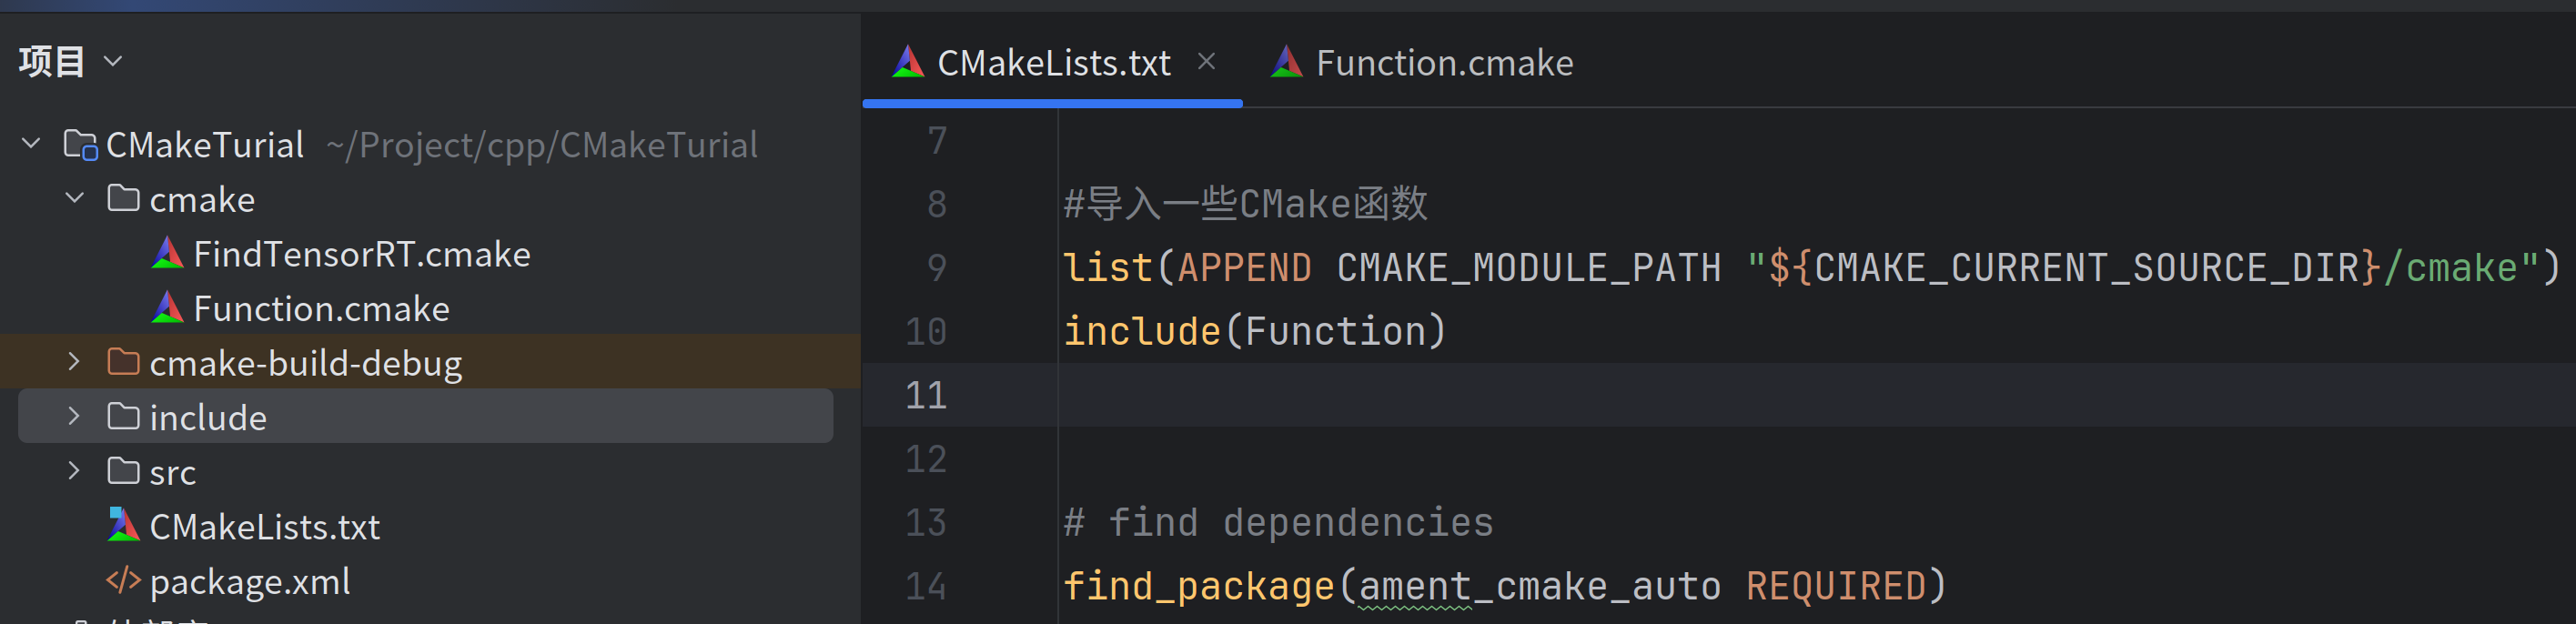
\includegraphics[width=0.7\textwidth]{cmake函数.png}
    \caption{实例项目结构} % 图片标题
    \label{fig:cmakeFunction} % 图片标签,用于引用
\end{figure}

这样,就可以在编译时打印出相关信息,方便调试。

\subsubsection{实例}

下面是一个实例项目的$CMakeLists.txt$文件,请试着读懂它:

\begin{tpython}
cmake_minimum_required(VERSION 3.8)
project(filter)

if(CMAKE_COMPILER_IS_GNUCXX OR CMAKE_CXX_COMPILER_ID MATCHES "Clang")
    add_compile_options(-Wall -Wextra -Wpedantic)
endif()

#导入一些CMake函数
list(APPEND CMAKE_MODULE_PATH "${CMAKE_CURRENT_SOURCE_DIR}/cmake")
include(Function)


# find_package 的高级平替,后面会讲
find_package(ament_cmake_auto REQUIRED)
ament_auto_find_build_dependencies()

###################项目目录设置######################
set(KALMAN_INCLUDE_DIR ${PROJECT_SOURCE_DIR}/include/kalman)
set(KALMAN_SRC_DIR ${PROJECT_SOURCE_DIR}/src/kalman)
set(MLS_INCLUDE_DIR ${PROJECT_SOURCE_DIR}/include/mls)
set(MLS_SRC_DIR ${PROJECT_SOURCE_DIR}/src/mls)
set(LMS_INCLUDE_DIR ${PROJECT_SOURCE_DIR}/include/lms)
set(LMS_SRC_DIR ${PROJECT_SOURCE_DIR}/src/lms)
set(EXEC_INCLUDE_DIR ${PROJECT_SOURCE_DIR}/include/exec)
set(EXEC_SRC_DIR ${PROJECT_SOURCE_DIR}/src/exec)

file(GLOB_RECURSE EXEC_SRCS ${EXEC_SRC_DIR}/*.cpp)
file(GLOB_RECURSE KALMAN_SRCS ${KALMAN_SRC_DIR}/*.cpp)
file(GLOB_RECURSE MLS_SRCS ${MLS_SRC_DIR}/*.cpp)
file(GLOB_RECURSE LMS_SRCS ${LMS_SRC_DIR}/*.cpp)

list(APPEND ALL_INCLUDE
        ${KALMAN_INCLUDE_DIR} ${MLS_INCLUDE_DIR} ${EXEC_INCLUDE_DIR} ${LMS_INCLUDE_DIR}
        ${OpenCV_INCLUDE_DIRS} ${EIGEN3_INCLUDE_DIR})

print_var(ALL_INCLUDE)

print_var(EXEC_SRCS)
print_var(KALMAN_SRCS)
print_var(MLS_SRCS)
print_var(LMS_SRCS)

include_directories(${ALL_INCLUDE})

##############静态库编译##################
add_library(filter_kalman ${KALMAN_SRCS})
add_library(filter_mls ${MLS_SRCS})
add_library(filter_lms ${LMS_SRCS})
list(APPEND FILTER_LIBS
        ${filter_kalman} ${filter_mls} ${filter_lms}
)
print_var(FILTER_LIBS)
############项目编译构建##########################
# add_executable的高级平替,以后会讲
ament_auto_add_executable(filter ${EXEC_SRCS})

target_link_libraries(filter ${OpenCV_LIBS} ${FILTER_LIBS})

# 这里进行项目的安装
if(BUILD_TESTING)
    find_package(ament_lint_auto REQUIRED)
    # the following line skips the linter which checks for copyrights
    # comment the line when a copyright and license is added to all source files
    set(ament_cmake_copyright_FOUND TRUE)
    # the following line skips cpplint (only works in a git repo)
    # comment the line when this package is in a git repo and when
    # a copyright and license is added to all source files
    set(ament_cmake_cpplint_FOUND TRUE)
    ament_lint_auto_find_test_dependencies()
endif()

# 神秘小代码,以后会讲
ament_auto_package()    
\end{tpython}

学了上面的内容,相信你已经可以写出自己的$CMakeLists.txt$文件了。


\section{ROS2基础}
在机器人开发过程中,我们往往需要使用到大量的传感器和执行机构,这时候,设备的有效管理和设备之间的通信就显得尤为重要,ROS2就是为了解决这一问题而生的。ROS2是一个开源的机器人操作系统,它提供了一系列的功能,包括:
\subsection{\textbf{引言:我们是如何从代码到机器人控制的}}
通过之前的学习,相信大家已经对如何再CMake的帮助下使用C++编写代码有了一定的了解。
之后你们会学习一些针对特殊需求的库,比如OpenCV、cuda等。他们能解决一些特定的问题,比如视觉处理
和模型运行等。

在此之前,你们需要学会如何把将要学的这些内容连接起来。比如,机器人的相机、传感器、MCU发来的信息会不断地
想你发送信息,我们需要一种“系统”能够从容地处理这些信息,对这些信息进行运算再发送出去。
这个“系统”其实就是操作系统(OS, Operating System)。对于个人计算机,我们使用的是Windows、Linux、Mac OS等,
他们帮我们进行了很多底层的工作,比如处理硬件、网络、驱动程序等。
而对于机器人来说,我们使用的是\textbf{ROS}(Robot Operating System),它帮助我们管理多个信息来源和不同信息,同时负责不同模块之间的通信。
这样一来,我们就不必要关注多个线程之间的同步、死锁等问题,只需要专注于业务逻辑的实现。
可以理解为如果不使用ROS2,我们需要自己使用C++的多线程库编写一个复杂的多线程系统,而ROS2可以替代你们上一章学的C++多线程,因为一个复多线程系统的编写
往往setTimeOut、wait等操作非常复杂,而ROS2使用DDS(Data Distribution Service)来实现通信,它已经帮我们处理了很多底层的细节。
\subsubsection{ROS2的版本}
和Linux与Ubuntu的关系类似,ROS2也有不同的版本或者说分支,比如ROS2 Foxy、ROS2 Eloquent等。
现在,我们队伍中主流使用的版本是\textbf{ROS2 Humble Hawksbill}。
\begin{figure}
    \centering
    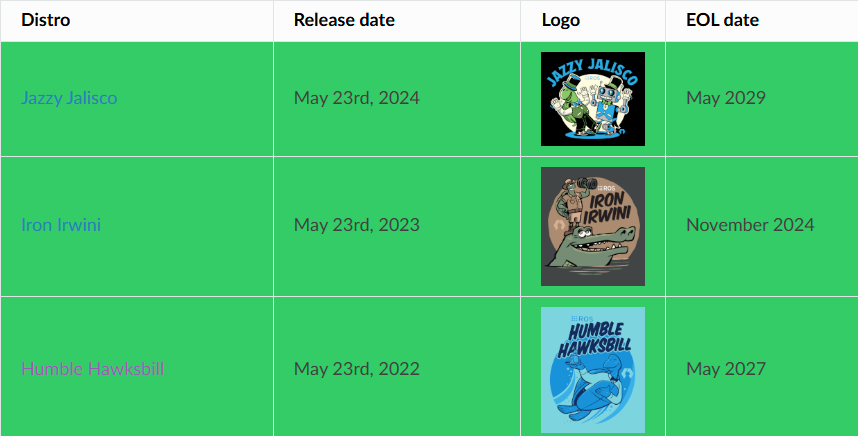
\includegraphics[width=0.8\textwidth]{Chapter4/img/ros2_logo.png}
    \caption{ROS2的最新版本跟新情况}
    \label{fig:ros2_logo}
\end{figure}

\subsubsection{ROS2的安装}

首先,我们需要安装ROS2的Humble Hawksbill 版本。
\begin{tbash}
    wget http://fishros.com/install -O fishros && . fishros
\end{tbash}
这条命令会帮你下载并运行一个脚本,根据它的引导选择下载ROS humble即可。
大概的输出为:
\begin{tbash}
    some output should be here...
\end{tbash}
这是一个非常好用的网站,江湖人称鱼香ROS。

这个命令在配置一个白板的Ubuntu系统时一般第一个运行,它会引导你更换系统源、安装必要的依赖包、配置环境变量等(甚至是下载QQ和微信)
这就减少了去官网上一个个寻找ubuntu版本的麻烦。

\subsection{ROS2架构}
\subsubsection{ROS2的系统架构}
ROS2的系统架构如下图所示:
\begin{figure}[h]
    \centering
    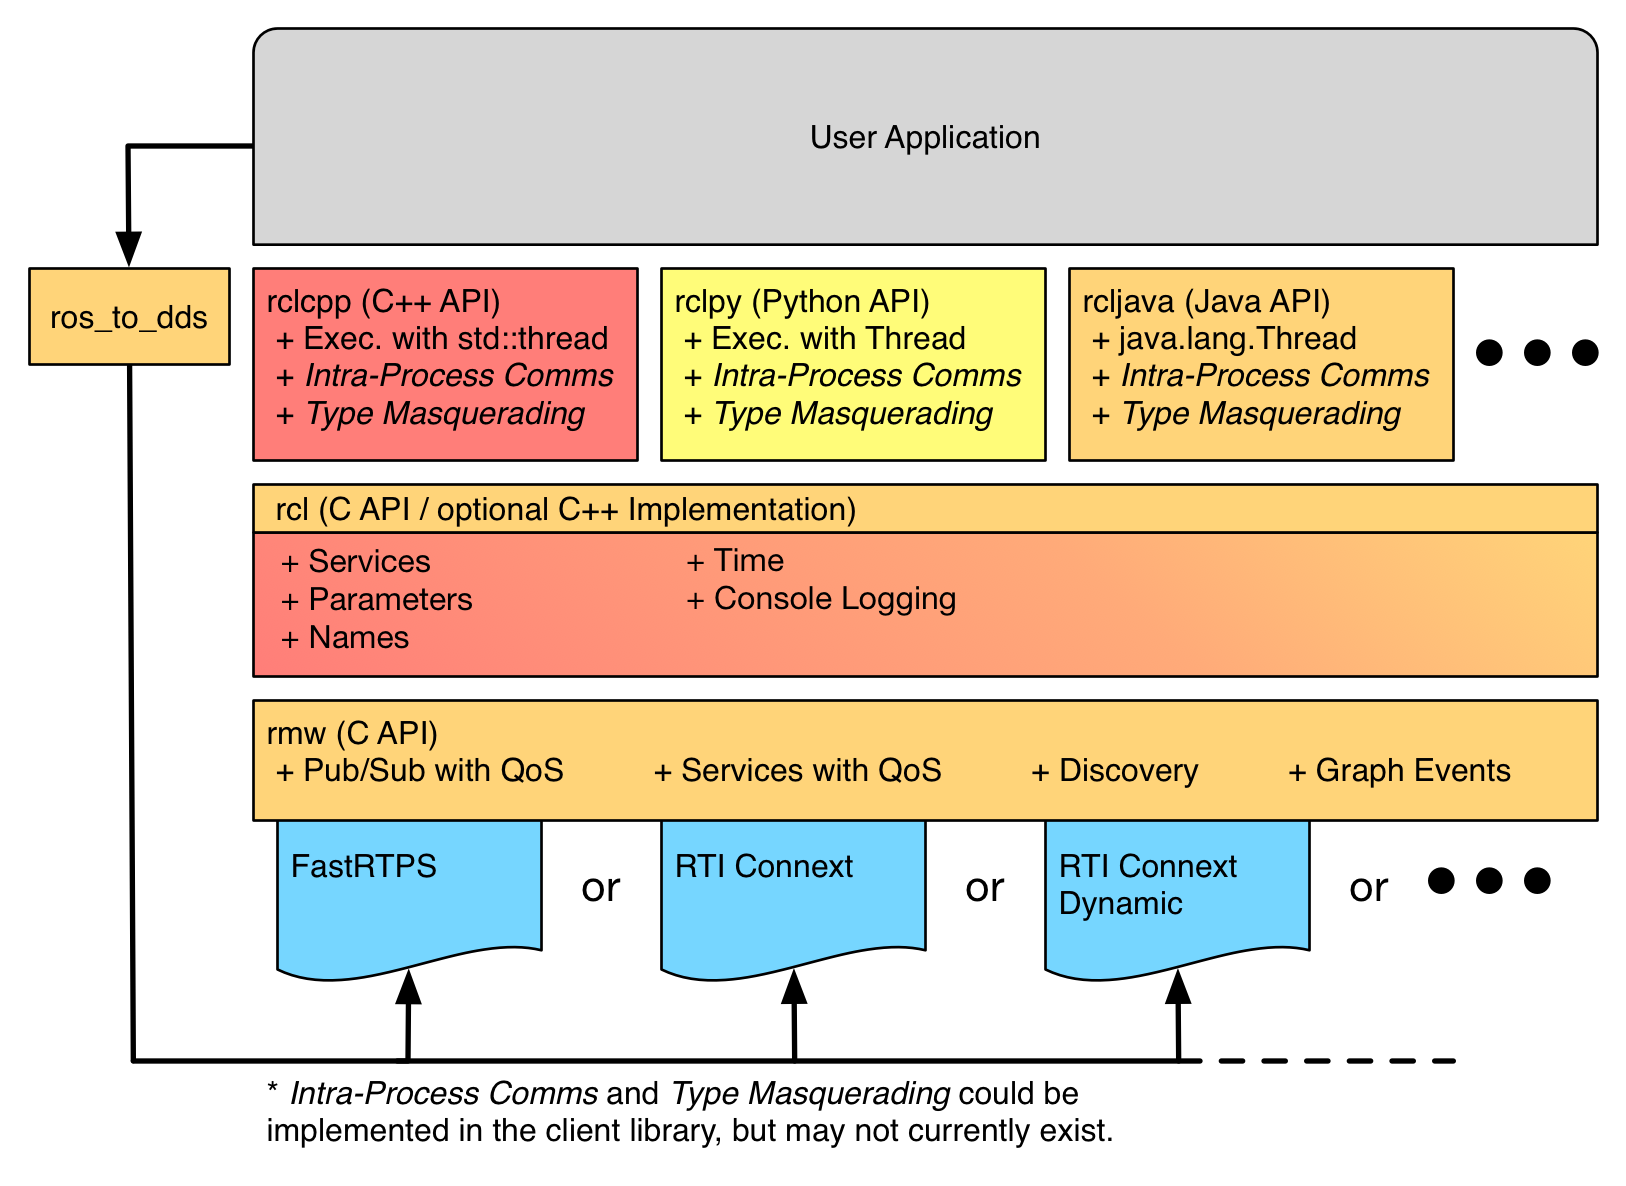
\includegraphics[width=0.8\textwidth]{Chapter4/img/ros2_arch.png}
    \caption{ROS2架构}
    \label{fig:ros2_arch}
    虽然你可能现在看不懂这个图,但不妨等学完之后再回过头来看看。
\end{figure}
一些需要听说过的属于的翻译:
\begin{itemize}
    \item \textbf{rclcpp}: ROS Client Library for C++,它是ROS2的C++客户端库,负责ROS2节点的创建、通信、生命周期管理等,我们使用的主要是这个库。
    \item \textbf{rmw}: ROS Middleware,它是ROS2的中间件,负责底层通信的实现。
    \item \textbf{Qos}: Quality of Service,它是ROS2的通信质量保证机制,用来控制通信的延迟、带宽等。
    \item \textbf{DDS}: Data Distribution Service,它是ROS2的分布式数据服务,用来实现ROS2节点之间的通信。
\end{itemize}
\subsubsection{ROS2的节点与组件}
\textbf{ROS2的基本思想是分布式的、模块化的。}

ROS2的节点是ROS2系统的基本单元,它可以包含多个ROS2组件。

我们可以用这个图来直观地理解ROS2的\textbf{节点}:
\begin{figure}[h]
    \centering
    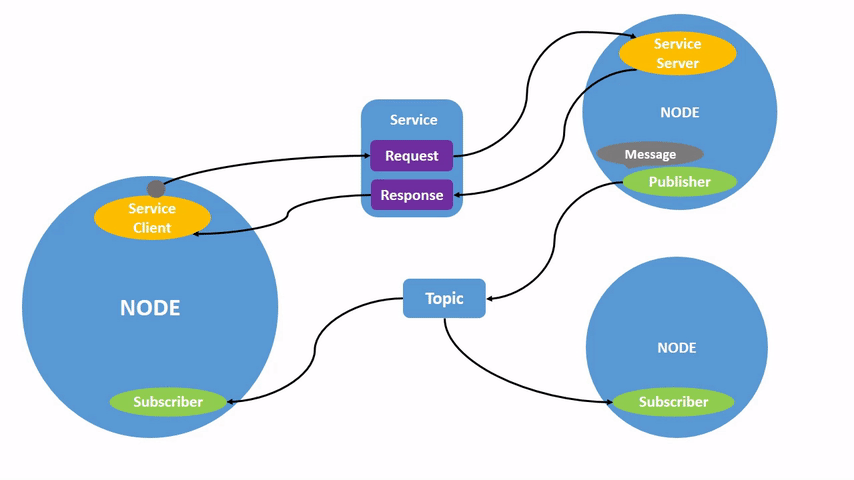
\includegraphics[width=0.8\textwidth]{Chapter4/img/ros2_node.png}
    \caption{ROS2节点与组件}
    \label{fig:ros2_node}
\end{figure}
这是一个动图,你可以去\underline{\href{https://docs.ros.org/en/humble/_images/Nodes-TopicandService.gif}{这里}}播放看看。

这个图直观的反映了ROS2的模块化是依靠\textbf{节点}完成的,节点的职责可以是接收某个传感器的信息(比如相机),也可以是对数据进行处理的流程(比如对相机的图像进行滤波),也可以是提供服务(比如反馈相机的参数信息)
当然这些功能也可以在一个节点中完成。同时可以注意到,节点之间的信息交流是依靠组件(Component)来实现的,一般来说一个节点的运行入口函数也是某个组件的回调函数。


对于我们实际上手操作的情况下,我们更感知的操作方式有两种。
一是使用CLI tools(command-line interface),二是使用Client Libraries。
我们一般使用CLI tools来创建、运行、调试节点,而Client Libraries则用于编写节点的逻辑。

\subsection{ROS2的节点}
ROS2的节点是ROS2系统的基本单元,它可以包含多个ROS2组件,比如发布者(Publisher)、订阅者(Subscriber)、服务(Service)、客户端(Client)等。
下面我们先从什么是节点开始介绍。

\subsection{ROS2}

https://design.ros2.org/articles/roslaunch.html

\section{OpenCV与图像处理基础}
在计算机处理过程中,图像处理是一种重要的任务。OpenCV是开源的计算机视觉库,它提供了一系列的图像处理算法,包括图像的读取、写入、显示、裁剪、缩放、旋转、滤波、轮廓检测、特征提取、匹配、形态学处理等。

\section{神经网络与深度学习基础}
机器学习是人工智能领域的一个重要研究方向,它利用大量的数据训练模型,从而对未知的输入进行预测。深度学习是机器学习的一个分支,它利用神经网络来学习复杂的非线性函数。

\subsection{了解神经网络}
如今神经网络在各个领域都有涉及, 在计算机视觉领域更是有极大的优越性。从机器学习再到深度学习,几乎已经形成一个完整的
技术体系并且仍然在高速发展。
通常来说,神经网络一般有以下三个作用:
\begin{enumerate}
    \item \textbf{预测}: 这通常是一维层面的,通过给予计算机一定量已有的数据(通常是多组自变量和因变量)拟合出一个合适的曲线(函数),当有新的自变量传入的时候,通过该曲线给出预测的结果
    \item \textbf{识别}: 这通常是二维层面的,同样是给予计算机一定量的二维图像,同时告诉计算机我们想要识别的图像主体,给予其标注,通过大量数据的学习让计算机能够准确识别任意图像中符合要求的部分
    \item \textbf{自然语言}: 通过给予海量的文本数据,使计算机能够理解、解释和生成自然语言,进行情感分析和语言推断。
\end{enumerate}
这些只是对作用的简单解释,具体过程要比这复杂的多。

无论是一维的预测还是二维的识别,从本质上来说,所谓\textbf{学习},就是不断调整神经网络内部参数使参数达到一种足够泛化也足够准确的大小,能够保证传入
的数据在经过这群参数组成的\textbf{“函数"}映射后,得到一个可信度高的答案。
那么在拟合这群参数后,如果没有处理好,会出现\textbf{欠拟合}和\textbf{过拟合}的问题

\begin{figure}[h]
    \centering
    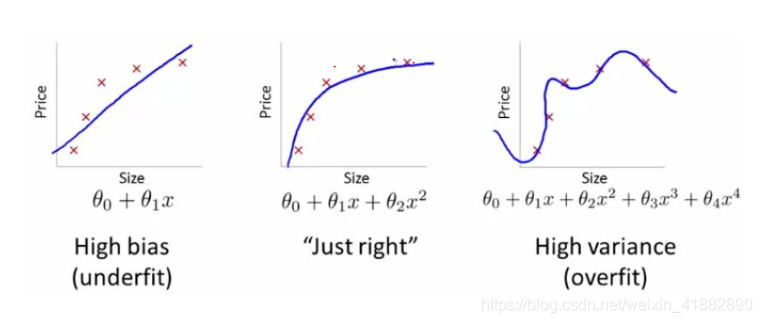
\includegraphics[width=0.8\textwidth]{拟合.png}
    \caption{欠拟合与过拟合}
    \label{fig:拟合}
\end{figure}

如图所示,欠拟合就是参数调整的太差了,根本没有预测的能力,得到的答案和实际上差距非常大,这时候我们就应该考虑增加训练数据或者
是增强数据的特征。

另一个过拟合,就是数据的特征过于明显或者是训练的过强导致网络没有足够的泛化能力,那么当传入的数据不是训练的数据的时候,将无法正确
预测,这时候就应该减少训练的次数,减少数据集的数量或者是降低数据的特征,提高泛化能力,

通过简单的了解,我们知道神经网络的作用以及神经网络是如何训练出来的,现在我们将通过自己动手搭建一个神经网络,在学习搭建的过程中对
更深入的内容进行讲述。
\subsection{动手搭建神经网络}
如果我们的网络只有简单的功能需求,那么用当今主流的pytorch就可以快速构建起一个神经网络,pytorch中封装好了很多搭建网络所需要的功能
我们只需要简单理解就能够直接调用使用。如果我们对准确性,效率等有更高的要求,可以使用已有的框架比如yolo,只需要准备好数据集和标注,按照需求
简单调整一下框架的参数,就可以训练出一个高性能的网络。

我们将从安装开始,一步步利用\textbf{pytorch}搭建出一个简单的识别图像中数字的网络。
\subsubsection{虚拟环境——Anaconda}
在安装Pytorch之前,我们要先安装Anaconda。

什么是Anaconda?一般来说在电脑上已经安装好了一个python环境,但是对于不同的项目需要不同的python环境
同时这些项目还要安装各种包和依赖,如果都把他们放在我们电脑最基础的环境下,很容易出现各种冲突问题而且很难管理。Anaconda能为我们创建不同的虚拟环境,
我们可以按照需要在这些虚拟环境里安装不同的包和依赖,它们不会相互影响,而且不同环境之间相互切换,操作简单,非常方便。同时Anaconda还有超过180个科学包和
依赖项,简单的几行命令就可以将这些包安装到指定的虚拟环境下,省去了麻烦的下载流程和令人头疼的配置过程。我们将用Anaconda创建一个独属于pytorch的虚拟环境。

Anaconda官方下载地址:\url{https://www.anaconda.com/download/}

按照官方流程安装好Anaconda后,在Windows的Anaconda Prompt(ubuntu的终端)输入
\begin{tbash}
    conda --version
\end{tbash}
如果显示版本号,说明安装成功。

\textbf{创建虚拟环境}

在Anaconda Prompt输入
\begin{tbash}
    conda create -n pytorch python=3.7
\end{tbash}
这样我们就创建了一个名为pytorch的虚拟环境,同时指定了python的版本为3.7,这样我们就可以在这个环境下安装pytorch了。

\textbf{激活虚拟环境}

在Anaconda Prompt输入
\begin{tbash}
    conda activate pytorch
\end{tbash}
我们会发现命令行前面多了(pytorch)字样,这就说明我们已经成功激活了pytorch环境。
这时输入
\begin{tbash}
    pip list
\end{tbash}
就可以看到当前环境下已经安装的包。
类似的
\begin{tbash}
    conda deactivate
\end{tbash}
就退出了当前环境。

\subsubsection{安装Pytorch}
在激活了pytorch环境后,我们就可以安装pytorch了。
在命令行输入
\begin{tbash}
    pip install pytorch torchvision
\end{tbash}
这样我们就安装好了pytorch,同时还安装了torchvision这个包是pytorch的辅助包,用于处理图像。
\textit{如果你出现了诸如网络问题导致无法安装,请改变虚拟环境的源为国内源,具体操作请自行搜索}

这样我们就安装好了pytorch-CPU,如果你有NVIDIA的显卡,可以考虑安装pytorch-GPU,网络的训练速度和推理速度会更快。
可以在命令行输入
\begin{tbash}
    nvidia-smi
\end{tbash}
查看自己的显卡型号,然后在官网上查看对应的CUDA版本,再安装对应的pytorch-GPU版本。
这里给上CUDA的官网下载地址:\url{https://developer.nvidia.com/cuda-toolkit-archive}
刚刚的pip install命令可以改为
\begin{tbash}
    pip3 install torch torchvision torchaudio --index-url https://download.pytorch.org/whl/cu{你的CUDA版本}
\end{tbash}

\subsubsection{搭建神经网络}
接下来用pytorch搭建一个简单的LeNet网络,识别MNIST数据集中的手写数字

选择一个你喜欢的IDE,比如VSCode, Pycharm, Clion等,创建一个python文件,选择解释器为刚刚创建的虚拟环境。
如果你感觉IDE的配置比较麻烦,也可以试试jupyter notebook,它是一个交互式的笔记本,可以直接在浏览器上运行代码,适合学习使用。

准备好后,首先导入需要的包
\begin{tpython}
    import torch
    import torch.nn as nn
    import torch.optim as optim
    import torchvision
    import torchvision.transforms as transforms
    import matplotlib.pyplot as plt
\end{tpython}
\begin{enumerate}
    \item torch: pytorch的核心包,包含pytorch的核心数据结构,以及所有的操作
    \item torch.nn: pytorch的神经网络包,包含所需的神经网络模块。
    \item torch.optim: pytorch的优化器包,包含了所有的优化器。
    \item torchvision: pytorch的图像处理包,包含了图像处理的所有操作。
    \item torchvision.transforms: pytorch的图像变换包,包含了所有的图像变换操作。
    \item matplotlib.pyplot: 画图的包,我们用来画出训练过程中的一些曲线。
\end{enumerate}

接下来准备MINST数据集

MINST数据集是一个包含了6万张训练图片和1万张测试图片的数据集,每张图片都是各式各样的手写的数组,每张图片上都有一个0-9的数字标签。
我们可以通过torchvision包中的datasets来下载这个数据集。
\begin{tpython}
    train_dataset = torchvision.datasets.MNIST(root='./data', train=True, transform=transforms.ToTensor(), download=True)
    test_dataset = torchvision.datasets.MNIST(root='./data', train=False, transform=transforms.ToTensor(), download=True)
\end{tpython}
这里的参数含义分别是:
\begin{enumerate}
    \item root: 数据集的存放路径
    \item train: 是否是训练集,True表示训练集,False表示测试集
    \item transform: 数据集的变换方式,这里是ToTensor(),将图片转换为tensor张量
    \item download: 是否下载数据集,如果已经下载过了,可以设为False
\end{enumerate}

但这里我们需要对数据集进行更多的转变操作,利用Compose将多个变换组合在一起,比如ToTensor()转化成Tensor和Normalize归一化
\begin{tpython}
    compose=torchvision.transforms.Compose([
        torchvision.transforms.ToTensor(),
        torchvision.transforms.Normalize((0.1307,), (0.3081,))
    ])

    train_dataset = torchvision.datasets.MNIST(root='./data', train=True, transform=compose, download=True)
    test_dataset = torchvision.datasets.MNIST(root='./data', train=False, transform=compose, download=True)
\end{tpython}

然后通过DataLoader加载数据集,使我们可以迭代访问数据集
\begin{tpython}
    train_loader = torch.utils.data.DataLoader(dataset=train_dataset, batch_size=64, shuffle=True)
    test_loader = torch.utils.data.DataLoader(dataset=test_dataset, batch_size=64, shuffle=False)
\end{tpython}
这里的参数含义分别是:
\begin{enumerate}
    \item dataset: 加载的数据集
    \item batch\_size: 一次加载的数据量, 这里是$64$
    \item shuffle: 是否打乱数据集
\end{enumerate}

我们完成了对数据集的准备,接下来搭建最基础最经典的LeNet网络结构:
\begin{figure}[H]
    \centering
    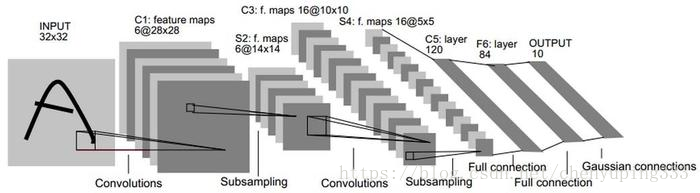
\includegraphics[width=0.7\textwidth]{images/LeNet.png}
    \caption{LeNet网络结构}
    \label{fig:LeNet}
\end{figure}

可以看到,除去输入层,LeNet一共有7层,按顺序进行卷积,池化,卷积,池化,全连接,全连接,全连接操作。

我们先对卷积,池化操作进行解释。

\textbf{卷积操作}:

卷积操作是神经网络中基本也是重要的操作之一,目的是提取图像的特征,通过一个n*n的卷积核在图像上滑动,将卷积核中心的像素大小替换为该卷积核上所有像素大小的加权和
\begin{figure}[H]
    \centering
    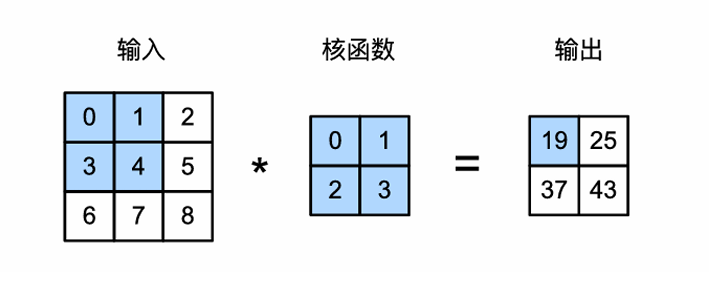
\includegraphics[width=0.7\textwidth]{images/卷积.png}
    \caption{卷积操作}
    \label{fig:卷积}
\end{figure}
用公式表示为:
\begin{equation}
    [H]_{i,j}=\sum_{a=-\Delta }^{\Delta}\sum_{b=-\Delta}^{\Delta}[V]_{a,b}[X]{i+a,j+b}   
\end{equation}
其中$[H]$是卷积后的图像,$[V]$是卷积核,$[X]$是原图像,$\Delta$是卷积核的大小。
这就是一次卷积层的操作。

我们要根据需要调整卷积核的大小,填充,步幅等参数。
\begin{enumerate}
    \item 卷积核大小: 通常是一个奇数,比如$3\times3$,$5\times5$,$7\times7$等
    \item 填充: 由于卷积核不是$1\times1$,所以边缘像素无法进行卷积,在多次卷积后,图像像素显著减少会失去许多信息,这就需要填充对图像进行扩充。
    \item 步幅: 卷积核每次滑动的步长,步长越大,卷积出的图像尺寸越小
\end{enumerate}
一般输出图像的形状为
\begin{equation}
    (n_{h}-k_{h}+p{h}+1) \times (n_{w}-k_{w}+p_{w}+1)
\end{equation}
其中$n_{h},n_{w}$是输入图像的高和宽,$k_{h},k_{w}$是卷积核的高和宽,$p_{h},p_{w}$是填充的高和宽。

\textbf{池化操作}:

池化操作是为了减少数据量,减少计算量,同时保留图像的主要特征,目的是减低卷积层对位置的敏感性。

汇聚层和卷积层相似,由一个池化核(池化窗口)在输入的信息上移动,同
样具有填充和步幅两个参数。汇聚操作计算的是窗口
中数据的最大值或者是平均值,这些操作分别称为\textbf{最大汇聚层}和\textbf{平均汇聚层}
\begin{figure}[H]
    \centering
    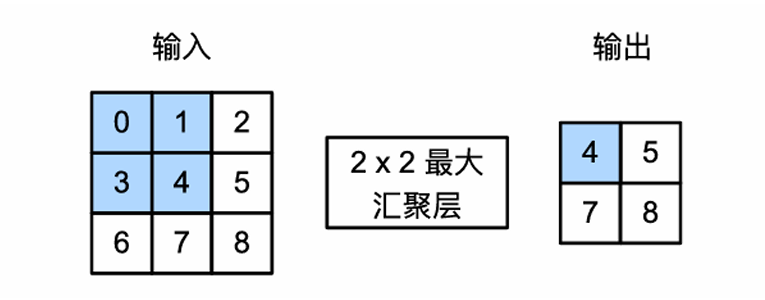
\includegraphics[width=0.7\textwidth]{images/池化.png}
    \caption{池化操作}
    \label{fig:池化}
\end{figure}

\textbf{全连接层}:

全连接层通常作为输出层使用,负责将网络的高层特征映射到最终的类别概率。
通常是为了整合特征,减少特征的维度,得到最终的输出类别。

\textbf{激活函数}:

这里我们涉及一下激活函数。
激活函数是神经网络中非常重要的一部分,它的作用是引入非线性因素,使得神经网络可以拟合任意复杂的函数。
通过加权和以及偏置来确定神经元是否应该激活,将输入信号转换为输出的
可微运算。大多数激活函数都是非线性的。
我们将主要用到ReLU激活函数,这是一个非常纯粹的函数:
\begin{equation}
    ReLU(x)=max(0,x)
\end{equation}
抛弃所有负元素,它求导表现得特别好:要么让参数消失,要么让参数通过

除此之外,还有sigmoid函数:
\begin{equation}
    sigmoid(x)=\frac{1}{1+\exp{-x}} 
\end{equation}
又称挤压函数,将($-\infty$,$\infty$)的任意数压缩到( $0$ , $1$ )

如此我们了解了神经网络的一些基本操作。

\textbf{搭建网络}:

首先写一个LeNet类,继承nn.Module
\begin{tpython}
    class LeNet(nn.Module):
        def __init__(self):
            super(LeNet, self).__init__()
            self.conv1=nn.Conv2d(1,6,5)
            self.pool1=nn.MaxPool2d(2,2)
            self.conv2=nn.Conv2d(6,16,5)
            self.pool2=nn.MaxPool2d(2,2)
            self.fc1=nn.Linear(16*5*5,120)
            self.fc2=nn.Linear(120,84)
            self.fc3=nn.Linear(84,10)
\end{tpython}

我们这里定义了LeNet类,并且在初始化函数中定义了一些层
显而易见
\textbf{卷积层}:
\begin{tpython}
    self.conv1=nn.Conv2d(3,16,5)
\end{tpython}
参数分别是\textbf{输入通道数,输出通道数,卷积核大小}。
我们知道图片是由RGB三个通道组成,因此这里输入通道数为3,按照LeNet的结构,让输出通道数为16,这是第一个卷积层。第二个卷积层同理,输入通道数为16,输出通道数为32。

\textbf{池化层}:
\begin{tpython}
    self.pool1=nn.MaxPool2d(2,2)
\end{tpython}
参数分别是\textbf{池化核大小,步幅}。
这里的池化核大小是2,步幅也是2,这是第一个池化层。第二个池化层同理。

\textbf{全连接层}:
\begin{tpython}
    self.fc1=nn.Linear(16*5*5,120)
\end{tpython}
参数分别是\textbf{输入特征数,输出特征数}。
输入特征数数根据上一层也就是池化层的输出决定。后面两个全连接层同理。
在最后一个全连接层我们输出10个特征,因为MNIST数据集中有10个类别(0 ~ 9)。

接下来我们定义前向传播函数,也就是网络的计算过程,处理输入数据,输出预测结果。
\begin{tpython}
    def forward(self, x):
        x=nn.relu(self.conv1(x))
        x=self.pool1(x)
        x=nn.relu(self.conv2(x))
        x=self.pool2(x)
        x=x.view(-1,16*5*5)
        x=nn.relu(self.fc1(x))
        x=nn.relu(self.fc2(x))
        x=self.fc3(x)
        return x
\end{tpython}
和上面的架构一样,只是在每次卷积操作后进行了激活操作,以及全连接层后进行了激活操作。
\textbf{x.view}:
这个函数是将一个多维的tensor转换为一维的tensor,参数-1表示自动计算,这里是将16*5*5的tensor转换为一维的tensor。
符合后面的全连接层输入。

如果想让网络每个处理更加简洁,可以使用\text{Sequential容器},将网络的层组合在一起。
比如我们可以将一次卷积,激活,池化操作组合在一起
\begin{tpython}
    self.conv1=nn.Sequential(
        nn.Conv2d(3,16,5),
        nn.ReLU(),
        nn.MaxPool2d(2,2)
    )
\end{tpython}
这样在forward函数中就可以直接调用这个容器,更加简洁。

这样我们就搭建好了一个简单的LeNet网络
\begin{tpython}
    Net=LeNet() 
\end{tpython}
实例化我们的网络

\textbf{定义损失函数:}

损失函数负责责量化实际值和预测值之间的差距,数值越小损失越小,因此我们通常要追求更小的损失。比如,平方误差函数
\begin{equation}
    l^{(i)}(\textbf{w},b)=\frac{1}{2}(\hat{y}^{(i)}-y^{(i)})^{2}
\end{equation}
$\hat{y}$表示预测值,$y$表示实际值,公式代表在$w$权重,$b$偏置下预测值和实际值的误差
一般情况下,我们要计算训练集上n个样本的平均损失L
\begin{equation}
    L(\textbf{w},b)=\frac{1}{n}\sum_{i=1}^{n}l^{(i)}(\textbf{w},b)
\end{equation}

在LeNet中我们使用\textbf{交叉熵损失函数}:
交叉熵公式:
\begin{equation}
    H(y,\hat{y})=-\sum_{i}y_{i}\log{\hat{y}_{i}}
\end{equation}
其中y是实际值,$\hat{y}$是预测值,交叉熵损失函数是一个非负函数,当预测值和实际值相等时,交叉熵为0,否则交叉熵越大,预测值和实际值差距越大。

代码中我们定义损失函数:
\begin{tpython}
    criterion=nn.CrossEntropyLoss()
\end{tpython}

\textbf{定义优化器:}

优化器负责更新网络的参数,使得损失函数最小化,这里我们使用\textbf{Adam优化器}:
Adam优化器是一种自适应学习率的优化器,它可以根据梯度的大小自动调整学习率,使得训练更加稳定。
所谓\textbf{学习率},就是每次更新参数的步长,学习率越大,参数更新的幅度越大,学习率越小,参数更新的幅度越小。
因此动态调整学习率有一定的重要性,降低梯度爆炸和梯度消失的风险。

\begin{tpython}
    optimizer=optim.Adam(Net.parameters(),lr=0.001)
\end{tpython}
这里的参数含义分别是\textbf{网络的参数,学习率}。Net.parameters()自带的函数,可以返回网络中所有的参数。

我们已经定义好了网络,损失函数,优化器,接下来我们就可以开始训练网络了。

\subsubsection{训练与测试网络}
在定义训练函数之前,我们需要了解一下网络训练过程中调整参数的主要方式——\textbf{反向传播}:

首先是\textbf{前向传播},前向传播是指从输入层到输出层的计算过程,通过输入数据,经过一系列的计算,得到输出结果。
这期间会储存一些中间变量,以便后续的反向传播。

反向传播是计算神经网络参数梯度的方法,该方法根据微积分中的\textbf{链式规则},按相反的
顺序从输出层到输入层遍历网络。该算法存储了计算某些参数梯度时所需的任何中间变量(偏导数)

在训练神经网络时,在初始化模型参数后,我们交替使用前向传播和反向传播,利用反向传播给出的梯度来更新模型参数。

\textit{反向传播需要利用前向传播中储存的中间值,因此我们一般需要保存这些中间值,这就导致需要更大的显存。
这些中间值的大小与网络层的数量和批量的大小大致成正比。
因此,使用更大的批量来训练更深层次的网络更容易导致\textbf{显存}不足(out of memory)错误}

就像前面所说的,神经网络训练本质上是调整参数,参数好坏的标准就是损失函数,我们要让损失函数尽可能的小,这其中用到了一个非常重要的算法——\textbf{梯度下降}:
梯度下降是一种优化算法,通过不断的往损失函数减小的方向上来更新参数以此降低误差,来达到优化模型的目的。
更新过程:
\begin{equation}
    (\textbf{w},b) \longleftarrow (\textbf{w},b) - \frac{\eta}{\left\lvert\mathcal{B}\right\rvert}\sum_{i\in\mathcal{B}}\partial_(\textbf{w},b)l^{(i)}(\textbf{w},b)
\end{equation}
\begin{enumerate}
    \item $\eta$: 学习率,控制参数更新的步长
    \item $\mathcal{B}$ : 批量大小,每次更新参数的样本数
    \item $\partial$ : 偏导数,迭代的是哪个参数就对哪个参数求偏导
    \item $l^{(i)}$ : 损失函数求得的损失
\end{enumerate}
这其中\textbf{学习率和批量}是手动设置的,是\textbf{超参数}。需要不断调整来达到最优效果。
在实际过程中,超参数的设置是十分关键的,这需要常年累月的调参经验。

\textit{算法只能使损失向最小值缓慢\textbf{收敛},无法在有限步数下准确求出最小值}

接下来我们定义train函数,用于训练网络
\begin{tpython}
    def train(epoch) # 传入当前的轮次
        running_loss=0.0 # 累加损失
        running_total=0 # 累加样本总数
        running_correct=0 # 累加正确样本数
        for batch_idx, data in enumerate(train_loader,0): # 遍历训练集
            inputs, labels=data # 获取输入和标签
            optimizer.zero_grad() # 梯度清零

            # forward + backward + optimize
            outputs=Net(inputs) # 前向传播
            loss=criterion(outputs,labels) # 计算损失
            loss.backward() # 反向传播
            optimizer.step() # 更新参数,优化

            running_loss+=loss.item() # 累加损失
            _, predicted=torch.max(outputs,dim=1) # 获取预测值
            running_total+=inputs.shape[0] # 累加样本总数
            running_correct+=(predicted==labels).sum().item() # 累加正确样本数

            if batch_idx % 300 == 299: # 不想要每一次都出loss, 选择每300次出一个平均损失, 和准确率
                print('[%d, %5d]: loss: %.3f , acc: %.2f %%'
                % (epoch + 1, batch_idx + 1, running_loss / 300, 100 * running_correct / running_total))
                running_loss = 0.0
                running_total = 0
                running_correct = 0
\end{tpython}

其中累加损失,累加样本总数,累加正确样本数是为了计算平均损失和准确率,这样我们可以更直观的看到网络的训练情况。
利用\textbf{enumerate}函数将train\_loader转换为一个迭代器,每次迭代返回一个batch的数据,同时返回一个索引,这样我们就可以知道当前是第几个batch。
\textbf{optimizer.zero\_grad()}是将梯度清零,因为pytorch默认会将梯度累加,所以每次迭代前都要清零。
然后经过前向传播获取到输出,将输出和标签传入损失函数,计算输出和标签之间的差距,也就是损失。
通过得到的损失,进行反向传播,更新网络中的参数,用优化器优化网络。

这样就完整的定义了一个训练函数,你也可以通过:
\begin{tpython}
    torch.save(model, f"../save/model_{epoch+1}.pth")
\end{tpython}
在指定路径下保存模型,以便后续使用。

\textbf{测试函数}:

训练完网络后,我们需要测试网络的性能,测试函数和训练函数类似,只是不需要反向传播和更新参数。
\begin{tpython}
    def test(epoch):
        correct=0 # 正确样本数
        total=0 # 总样本数
        with torch.no_grad(): # 测试集不需要算梯度
            for data in test_loader:
                images, labels=data # 获取输入和标签
                ouputs=Net(images)
                _, predicted=torch.max(outputs,dim=1)
                total+=labels.size(0)
                correct+=(predicted==labels).sum().item()
        acc=correct/total
        print('[%d / %d]: Accuracy on test set: %.1f %% ' % (epoch + 1, EPOCH, 100 * acc))  # 求测试的准确率,正确数/总数
\end{tpython}
测试函数和训练函数类似,只是获取在不需要梯度的情况下进行的。
correct和total是用来计算正确率的,方便我们看到网络的性能。

这样就定义了一个测试函数,接下来只需要在主函数中调用这两个函数,就可以训练和测试网络了。
\begin{tpython}
    if __name__ == '__main__':
        for epoch in range(50):
            train(epoch)
            test(epoch)
\end{tpython}

到此,成功完成了LeNet网络的训练和测试。这并不是一个很复杂的网络,但是确实包含了当今主流网络的主要操作。
当今网络的发展已经非常成熟,有很多优秀的网络结构,比如VGG,ResNet,DenseNet等,这些网络结构都有自己的特点。
它们都是基于LeNet的基础上不断发展而来,通过不断的尝试和改进,才有了现在的网络结构。
如果你掌握了LeNet的基本操作,那么学习其他网络结构就会变得更加容易。

\subsubsection{模型的导出和使用}
我们利用torch.save()函数将模型保存下来后,可以在其他地方加载模型,继续训练或者是直接使用。

\textbf{模型的使用:}
\begin{tpython}
    model=torch.load('model.pth')
    model.eval() # 将模型设置为评估模式
    with torch.no_grad():
        output=model(input) # 得到输出
        print(output)
\end{tpython}

\textbf{\textit{*利用GPU加速训练:}}

如果你有NVIDIA显卡,并且按照上面的步骤安装了pytorch-GPU版本,只需要在代码中简单加几行代码,就可以实现在
GPU上训练我们的模型。由于显卡的特性,GPU运算过程中,需要指令和数据都存储在显存中。
对于我们的神经网络就是,将网络结构,损失函数和数据都加载到显存中,然后进行运算。
可以使用$.cuda()$函数将模型加载到GPU上,然后在训练过程中,将数据也加载到GPU上进行运算,
使用$.to('cpu')$将数据转移到内存中,便于后续的处理。
GPU相比于CPU牺牲了大部分在CPU上属于缓存区等区域的面积,用来放更多的运算核心,因此GPU比
CPU更适合并行运算,运算速度更快,更适合网络模型训练,去处理大量的数据。

比如在代码中,我们加上
\begin{tpython}
    # model声明后
    model.cuda()
    ....
    ....
    # train函数中
    inputs, labels=data
    inputs=inputs.cuda()
    labels=labels.cuda()
    ....
    ....
    # test函数中
    images, labels = data
    images = images.cuda()
    labels = labels.cuda()
    
    # 在损失函数下也可以加上
    loss_function = loss_function.cuda()
\end{tpython}
再次训练,你会发现训练速度大大提升,从loss的输出就可以看出。

\textbf{\textit{*关于YOLO等框架:}}

YOLO是一个非常优秀的目标检测框架,它的全称是You Only Look Once,它的特点是速度快,准确率高,适合实时目标检测。
YOLO如今仍然在不断迭代更新,如今已有诸如YOLO-v5,YOLO-v8,YOLO-v10等一系列的版本。
其支持不同功能模型的训练,比如detect(检测),classify(分类),pose(姿态估计)等。

\begin{figure}[H]
    \centering
    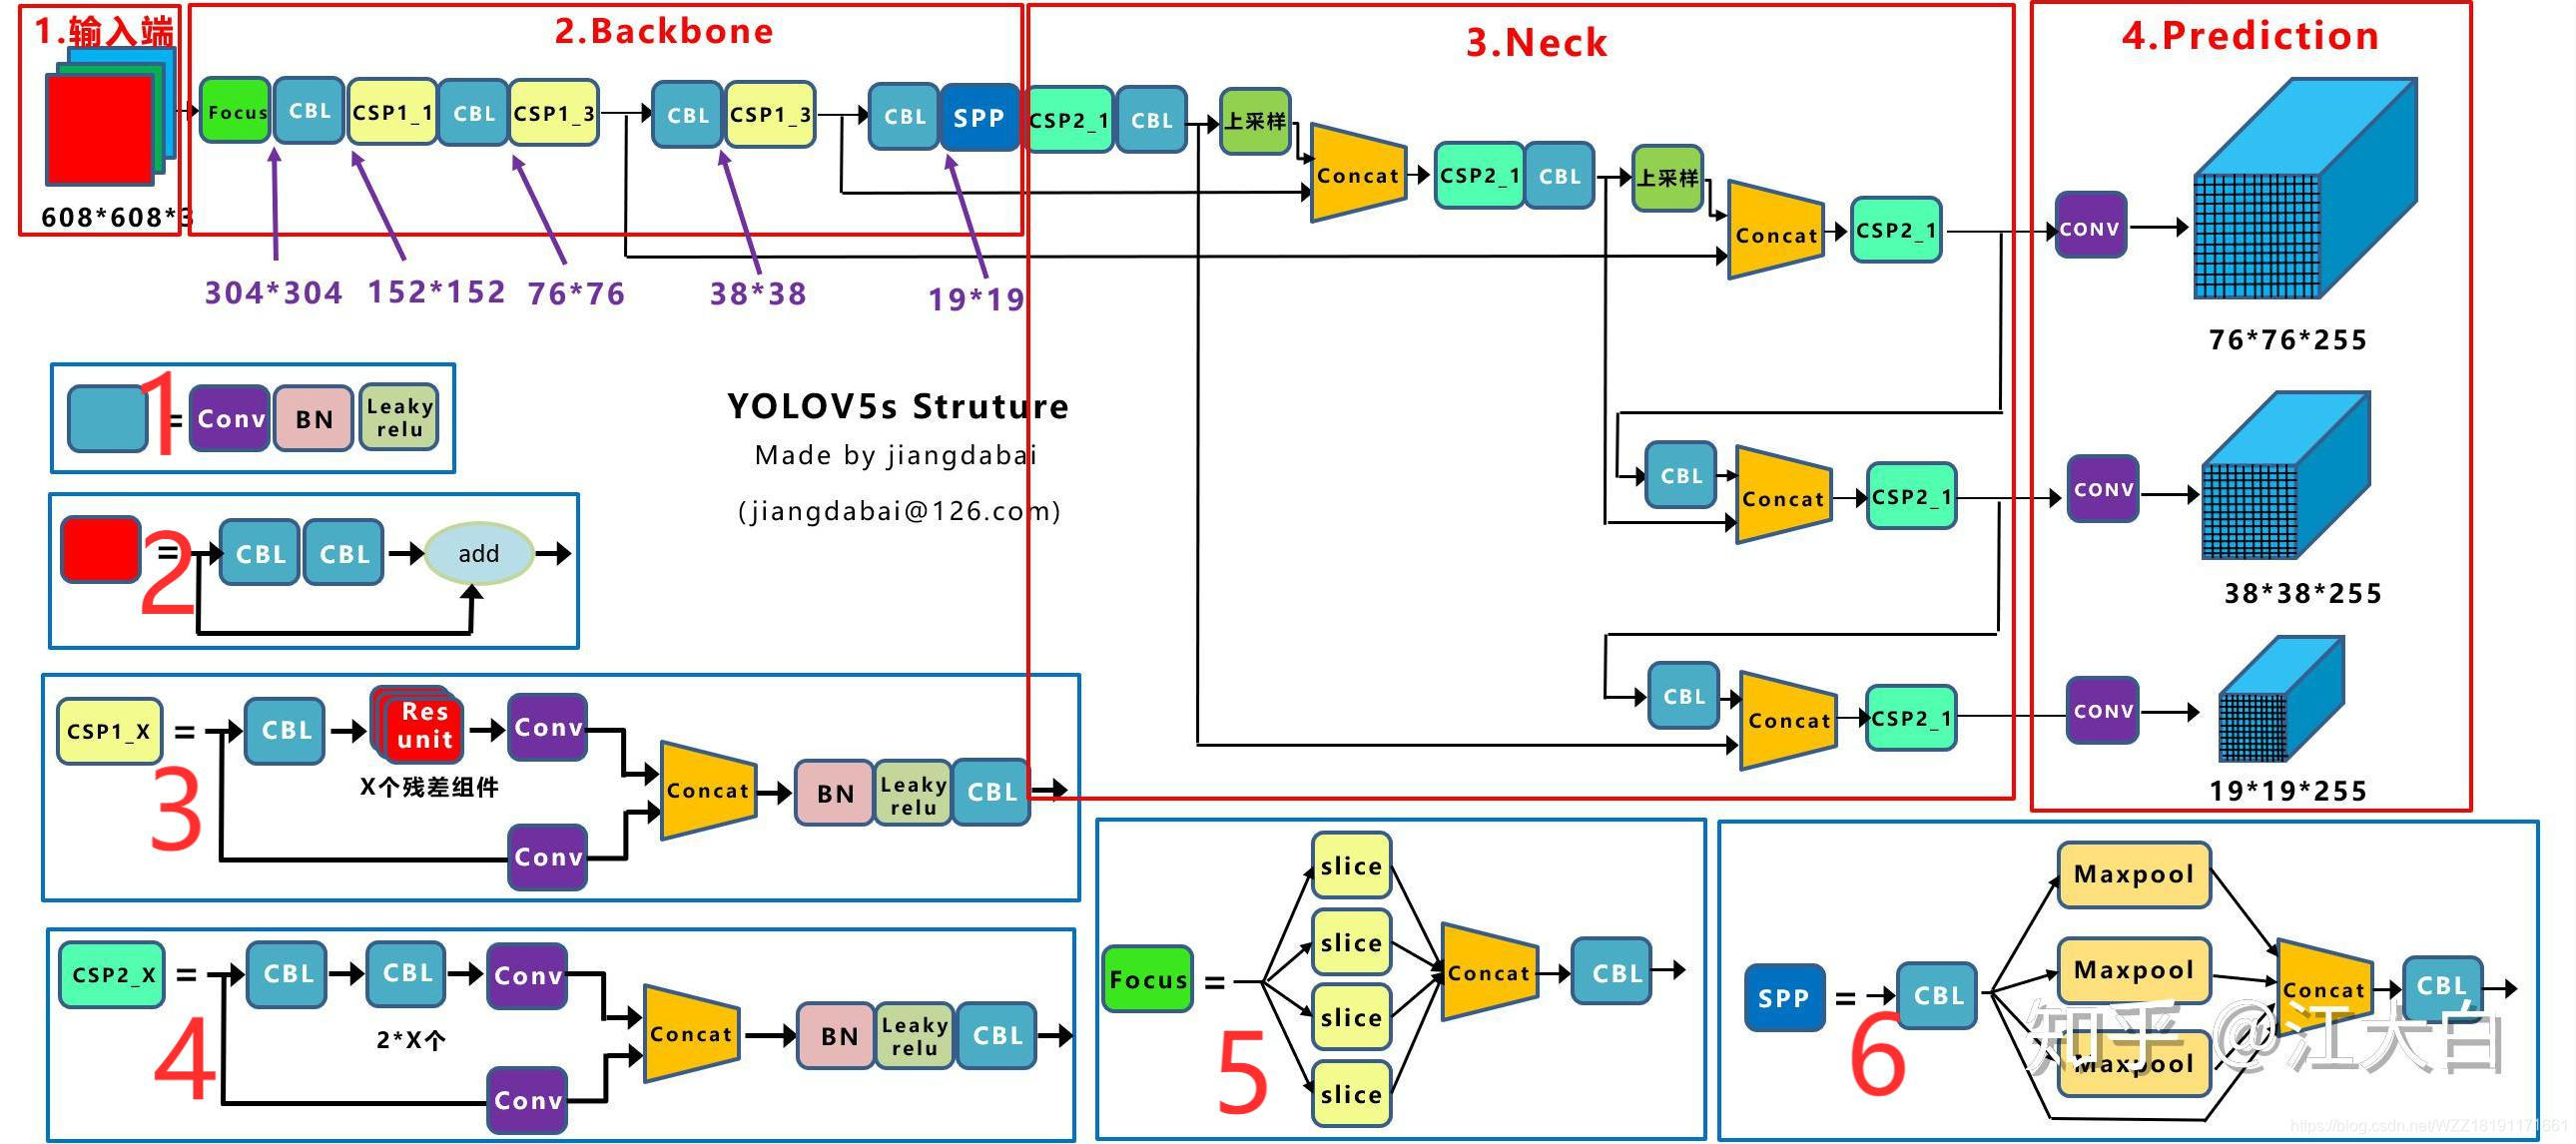
\includegraphics[width=0.8\textwidth]{images/YOLOv5.jpeg}
    \caption{YOLOv5网络架构}
    \label{fig:YOLOv5}
\end{figure}

可以通过这里了解:\url{https://github.com/THU-MIG/yolov10}

\url{https://blog.csdn.net/WZZ18191171661/article/details/113789486}

\subsection{简单了解模型部署}
如果我们已经拥有了一个训练好的模型,但是事实上这并不能草草的生搬硬套在我们实际的项目中。
一个项目通常不会是在拥有着高性能的NVIDIA显卡和高性能的CPU上运行的,通常是在一些性能较低的设备上,比如
在机器人上,代码运行在minipc,而minipc的性能和配置有限(intel旗下的nuc甚至没有GPU),因此我们需要尽量激发设备的性能,提高模型的推理速度。
这就要涉及到模型的部署。

\begin{enumerate}
    \item \textbf{CPU上的模型部署}: intel官方提供了一个完整的开源的部署工具——openvino,利用openvino提供的C++接口,可以将训练好的模型转换为openvino支持的模型,然后在CPU上运行,可以大大提高模型的推理速度。
    \item \textbf{GPU上的模型部署}: NVIDIA也提供了一个完整的开源的部署工具——tensorRT,同样也可以利用相应的API使得模型在GPU上实施推理,拥有更快的推理速度.
\end{enumerate}

\textbf{\textit{*有关模型文件类型:}}

模型文件的类型并不是单一的,不同的框架支持的是不同的文件类型。
譬如pytorch导出的模型为.pth文件,YOLO框架导出的是.pt文件。
而在openvino部署模型的时候,又需要把模型转换没xml和bin文件。
tensorrt所需的又是.engine文件。

模型文件类型的不同确实是一件麻烦的事情,因此领域内出现了一种.onnx文件,它使得不同的深度学习框架之间可以互操作。
openvino和tensorrt都支持对onnx文件的转换。有相应的API可以将onnx文件转换为自身所需要的文件类型。YOLO官方也给出了
相关的指令能够一键转换将.pt转换为.onnx文件。onnx文件就像是一个中间文件,使得不同框架之间的转换变得更加容易。

\textit{如果你有一个ONNX文件,你可以访问网站:\url{https://netron.app/}查看ONNX文件的结构,方便了解模型的结构}

\subsection{总结}
对于当今的科研工作相关人员来说,神经网络是不得不去学习的领域,同样也是一个非常重要的领域。
AI已经走进了我们的生活,无论是在自动驾驶,人脸识别,语音识别等领域,AI都有着广泛的应用。
在我们机器人的自瞄系统中,识别装甲板上的数字,识别敌方机器人,识别装甲板; 以及雷达系统,都有神经网络的身影。
感兴趣的同学可以多多学习,多多实践,祝大家学有所成。

\section{CUDA与GPU加速基础}
GPU是一种并行计算平台,它可以加速计算机的计算任务。CUDA是一种基于GPU的编程语言,它可以用来编写高性能的并行程序。

\section{相机参数与成像原理*} 

在机器视觉算法中,有一个很重要又经常被忽略的部分。有些时候我们太关注算法的性能,但是忽略了相机的成像质量。“巧妇难为无米之炊”,如果相机成像的效果不好,那么再优秀的算法都无法发挥作用。
相机是机器视觉最重要的组成部分,它可以捕捉到周围环境的各种信息,并将其转换为图像。相机参数是相机的一些基本参数,如焦距、光圈、快门等。
了解相机参数和成像原理对于理解相机的工作原理非常重要。

\section{信号处理与滤波器*}
在前端的成像和识别过程中,由于或多多少的原因,信号会发生一些变化,也会产生大量的噪声。如何滤除这些噪声,对于算法决策的准确性至关重要,在本章节我们将学习一些滤波器的基本知识。
并且运用我们学习到的知识,去自主设计一些滤波器,并将其应用到我们的算法中。

\section{导航技术初步*}
对于一个智能机器人来说,获取周围环境和自身情况的能力是至关重要的。导航技术是其核心技术之一。在本章节中,我们将了解激光雷达的工作原理,并学习一些基本的导航算法,并将其应用到我们的机器人中。

\section{\quad 决策树算法*}
在机器学习领域,决策树算法是一种常用的算法,它可以使得机器人可以灵活地对外界环境做出正确的响应。在本章节中,我们将学习决策树算法的基本原理,并将其应用到我们的机器学习项目中。

\bibliographystyle{plain} % 选择参考文献的样式
\bibliography{ref} % 指定BibTeX文件


\end{document} 